\documentclass[12pt]{amsart}
\usepackage[T1]{fontenc}
\usepackage[utf8]{inputenc}

\usepackage[top=1.95cm, bottom=1.95cm, left=2.35cm, right=2.35cm]{geometry}

\usepackage{hyperref}
\usepackage{enumitem}
\usepackage{tcolorbox}
\usepackage{multicol}
\usepackage{fancyvrb}
\usepackage{amsmath}
\usepackage[french]{babel}
\usepackage[
    type={CC},
    modifier={by-nc-sa},
	version={4.0},
]{doclicense}
\usepackage{textcomp}
\usepackage{tcolorbox}
\usepackage{tnsmath}

    
\newtheorem{fact}{Fait}%[section]
\newtheorem*{theorem}{Théorème}
\newtheorem{example}{Exemple}[section]
\newtheorem{remark}{Remarque}[section]
\newtheorem*{proof*}{Preuve}

\setlength\parindent{0pt}


\DeclareMathOperator{\taille}{\text{\normalfont\texttt{taille}}}

\newcommand\sqseq[2]{\fbox{$#1$}_{\,\,#2}}

\newcommand\floor[1]{\left\lfloor #1 \right\rfloorx}


\DefineVerbatimEnvironment{rawcode}%
	{Verbatim}%
	{tabsize=4,%
	 frame=lines, framerule=0.3mm, framesep=2.5mm}
	 
	 
	 
\begin{document}

\title{BROUILLON - Un simple (\!?) billard à deux bandes - Ajouter lien acvec PI : 3blue1brown galperin}
\author{Christophe BAL}
\date{25 Déc. 2018}

\maketitle

\begin{center}
	\itshape
	Document, avec son source \LaTeX, disponible sur la page
	
	\url{https://github.com/bc-writing/drafts}.
\end{center}


\bigskip


\begin{center}
	\hrule\vspace{.3em}
	{
		\fontsize{1.35em}{1em}\selectfont
		\textbf{Mentions \og légales \fg}
	}
			
	\vspace{0.45em}
	\doclicenseThis
	\hrule
\end{center}



\setcounter{tocdepth}{2}
\tableofcontents



\section{Présentation du problème}

Notre billard est un peu bizarre car il est juste constitué de deux demi-droites de même origine, et notre bille est dans le secteur angulaire le "plus petit" formé par ces deux bandes. Ceci se représente comme suit.

\medskip

\begin{center}
	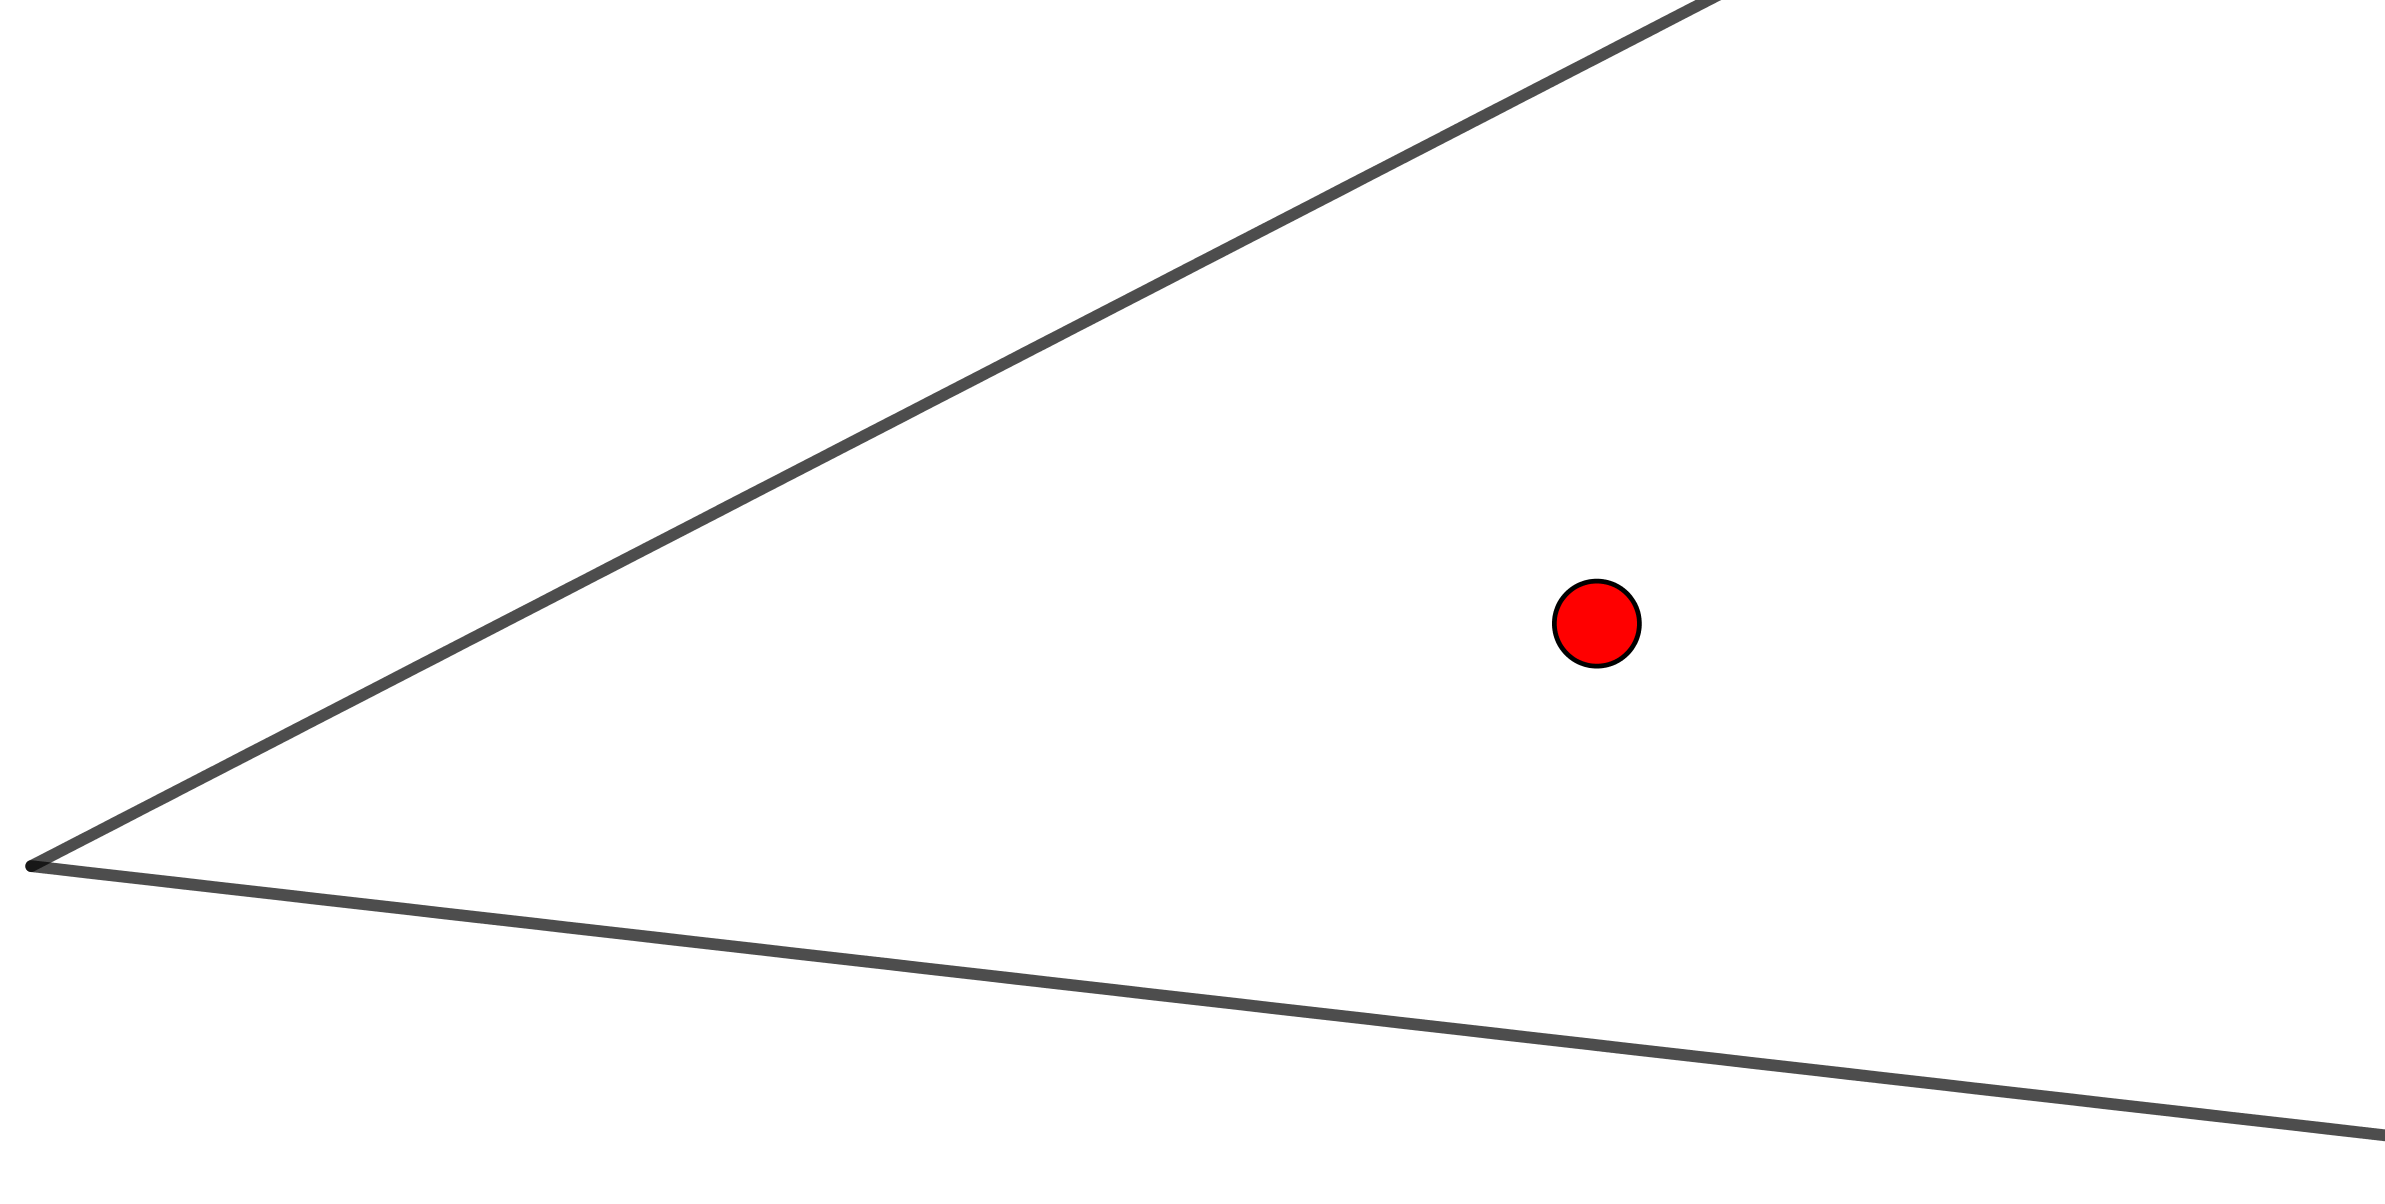
\includegraphics[width=12cm]{basic-math-pool/empty.png}
\end{center}

Dans la suite, nous considérons que notre bille est en fait un point, et du coup nous ne considérons pas les effets de rotation de la bille, et de plus nous ignorons les frottements, autorisant ainsi la bille à se balader vers l'infini et au-delà \emph{(tout ceci pour plus de réalisme)}.

\medskip

Concrètement, on pourrait se munir de deux miroirs plans verticaux et d'une source pouvant envoyer, dans un plan horizontal, un rayon laser dans une direction donnée.


\section{Rechercher et conjecturer}

Ci dessous, sur le cercle trigonométrique associé à un repère orthonormé $\paxes{O | I | J}$ , nous avons placé, les points $A$ , $B$ et $S$ de sorte que $\angleorient{\vect{OI}}{\vect{OS}} = \angleorient{\vect{OI}}{\vect{OA}} + \angleorient{\vect{OI}}{\vect{OB}}$ \emph{(cette construction est très naturelle)}.
Sauriez-vous conjecturer
\footnote{
	Le lieu de téléchargement de ce document contient un fichier GeoGebra \texttt{base-tool.ggb} manipulable dynamiquement pour vérifier combien il est aisé de conjecturer quelque chose.
}
un moyen simple de construire le point $S$ à partir des points $A$ et $B$ \emph{(la réponse est donnée dans la page suivante)} ?


\medskip

\begin{multicols}{2}
	\center

	\fbox{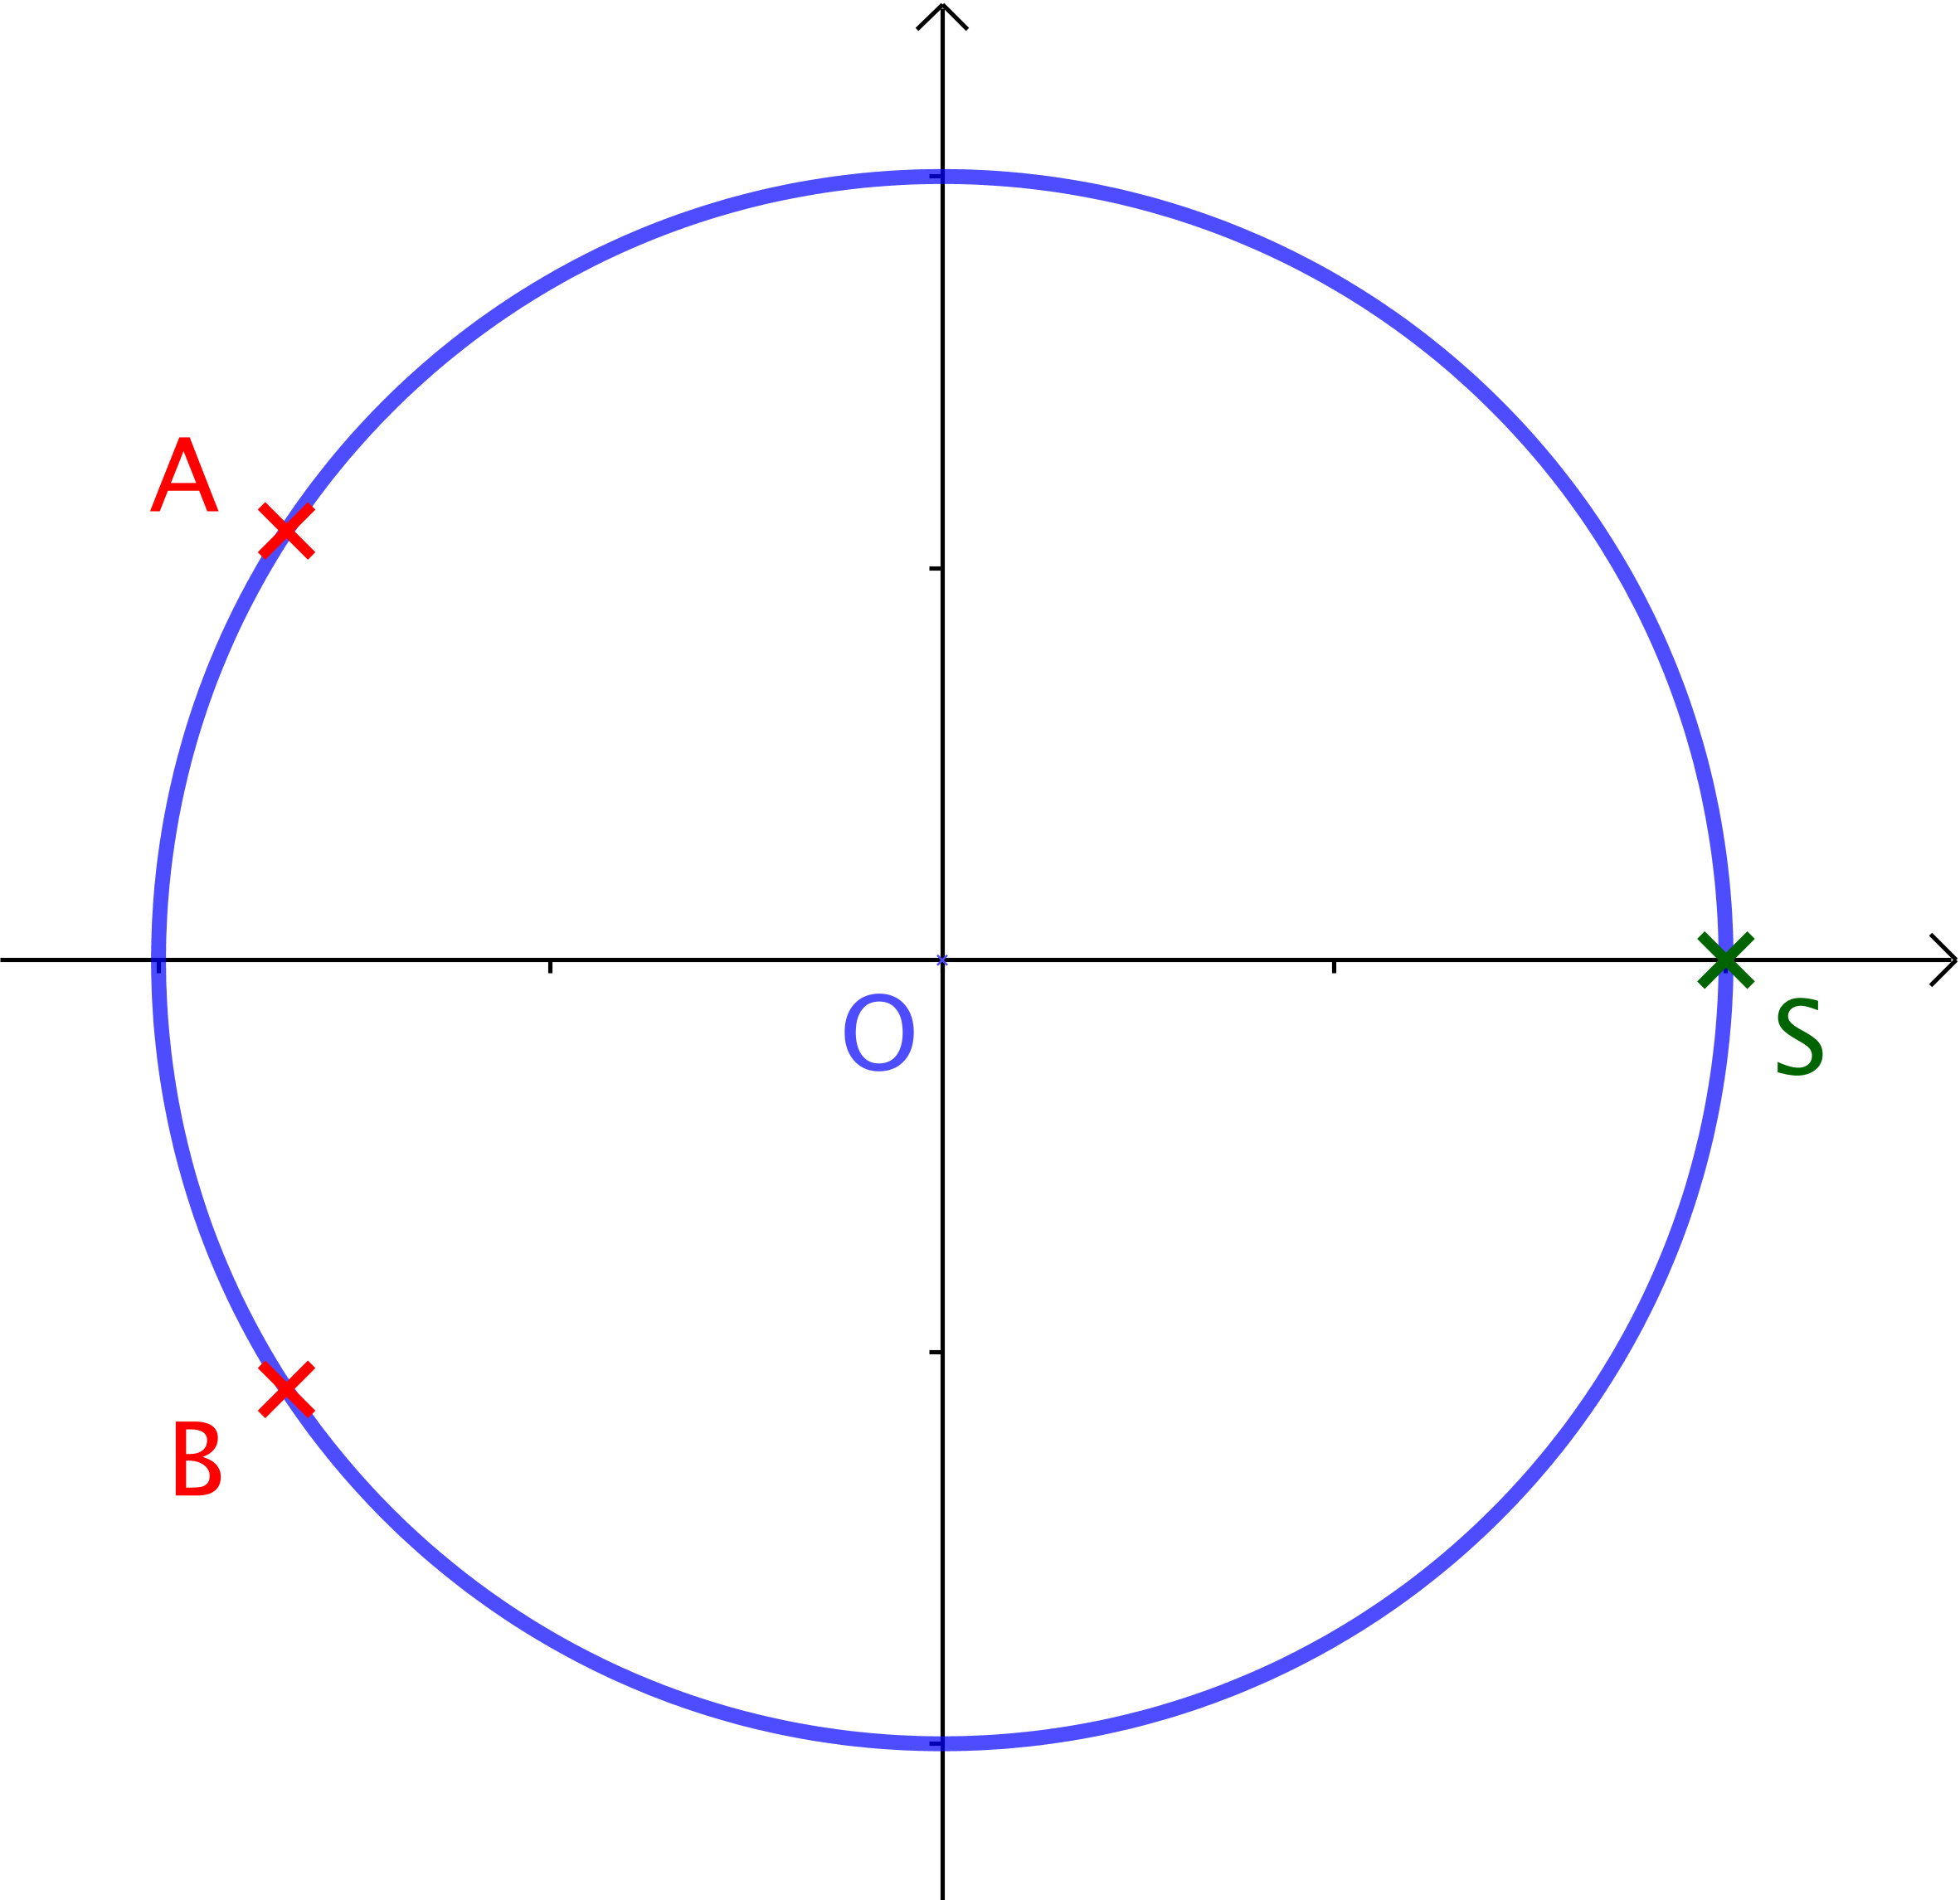
\includegraphics[scale = .75]{addition-on-ellipsis/conjecture/h-sym.png}}

	\columnbreak

	\fbox{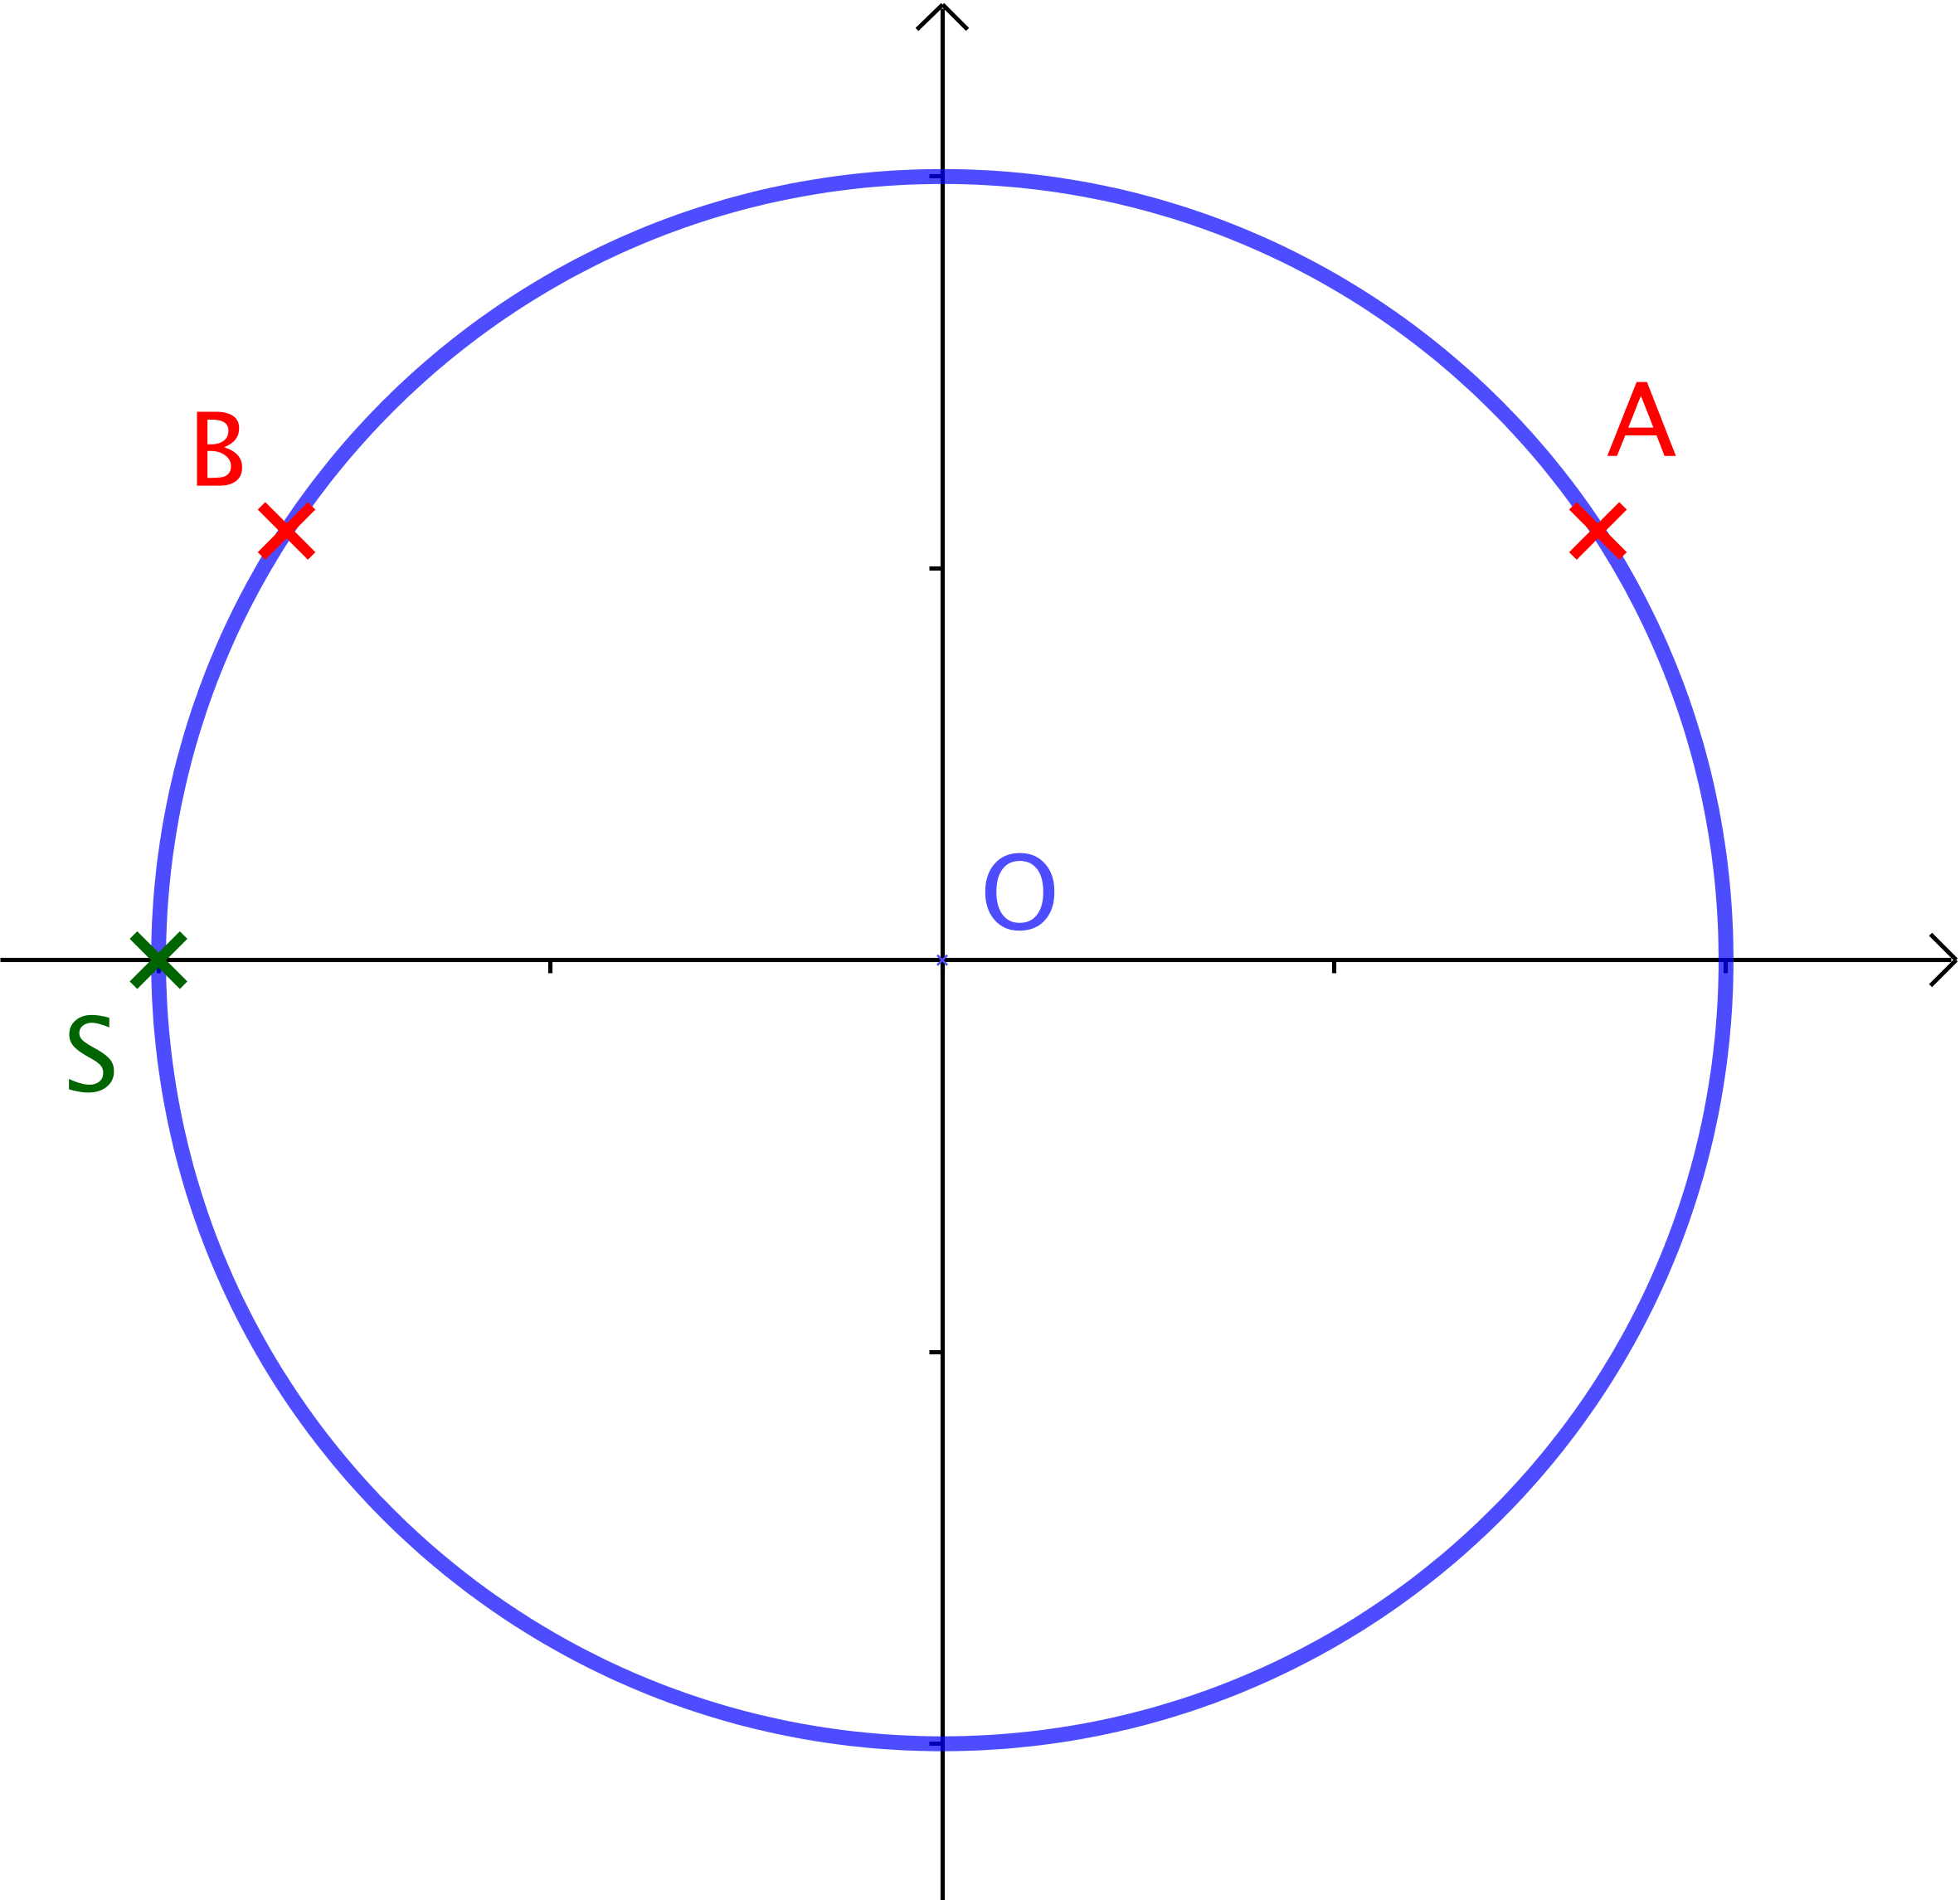
\includegraphics[scale = .75]{addition-on-ellipsis/conjecture/v-sym.png}}
\end{multicols}


\medskip

\begin{multicols}{2}
	\center

	\fbox{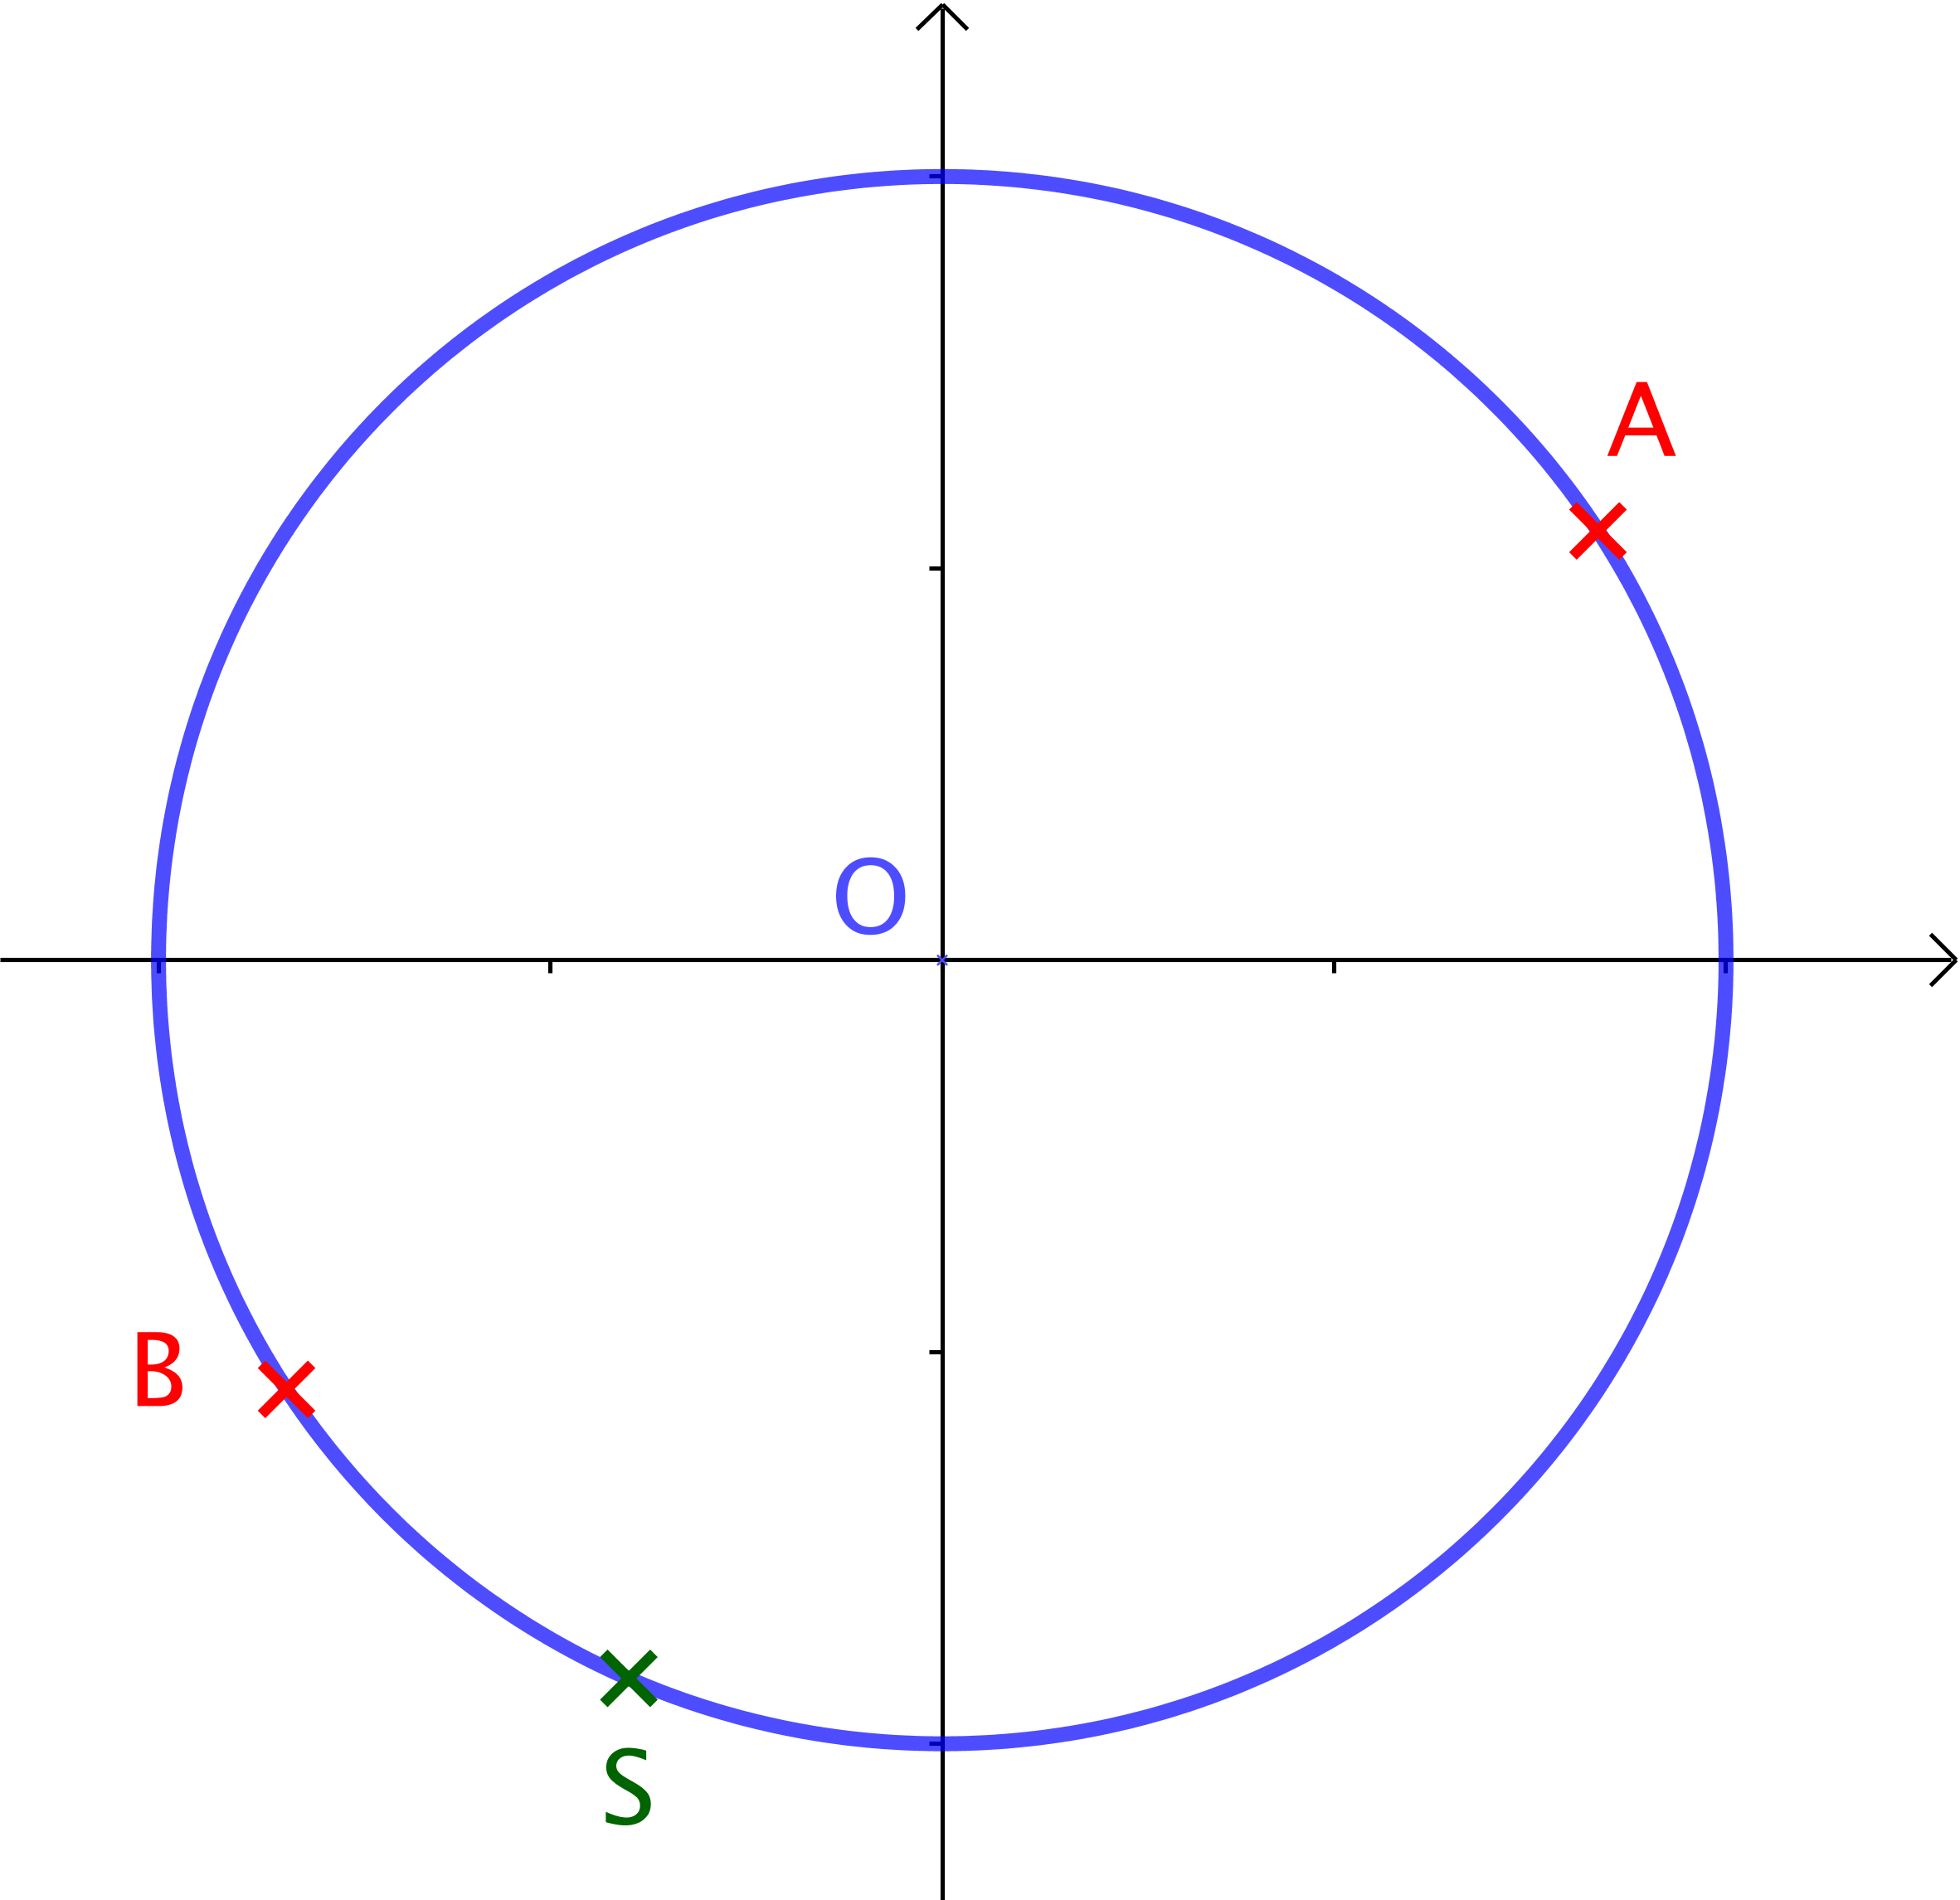
\includegraphics[scale = .75]{addition-on-ellipsis/conjecture/O-sym.png}}

	\columnbreak

	\fbox{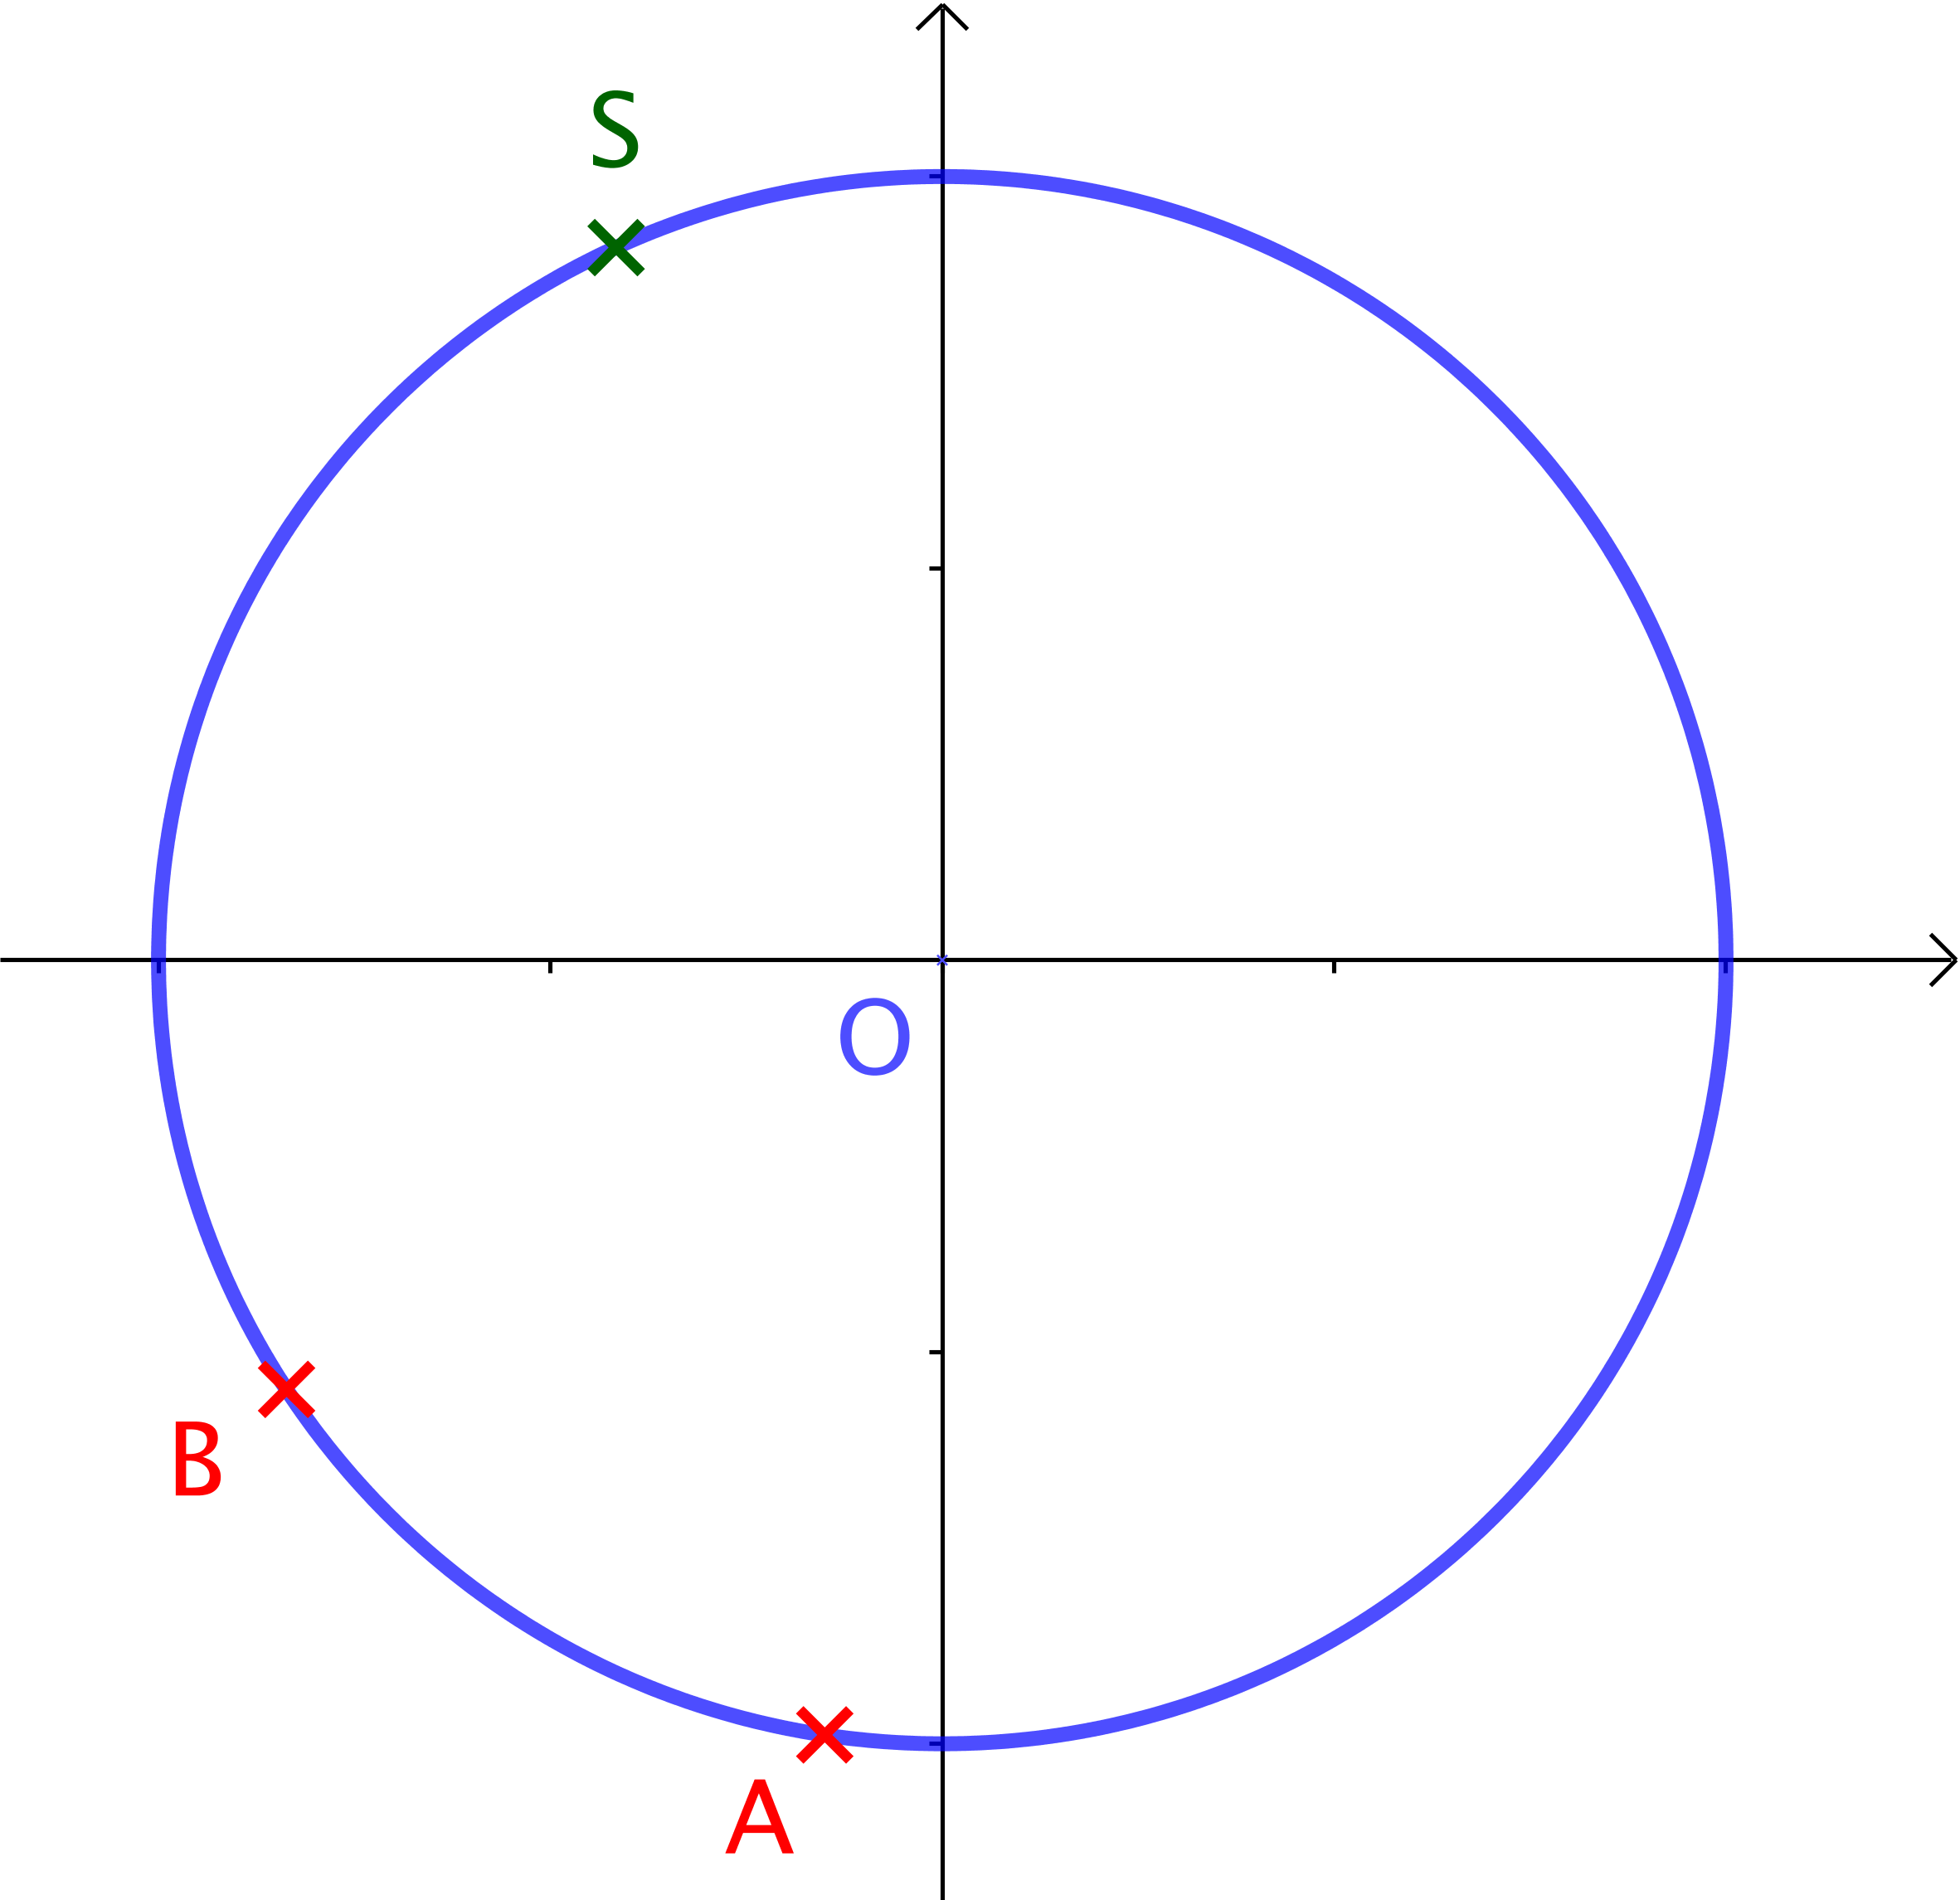
\includegraphics[scale = .75]{addition-on-ellipsis/conjecture/general.png}}
\end{multicols}


\newpage

Pour mieux voir ce qu'il se passe, il suffit de tracer quelques droites. Voici ce que cela donne.

\begin{multicols}{2}
	\center

	\fbox{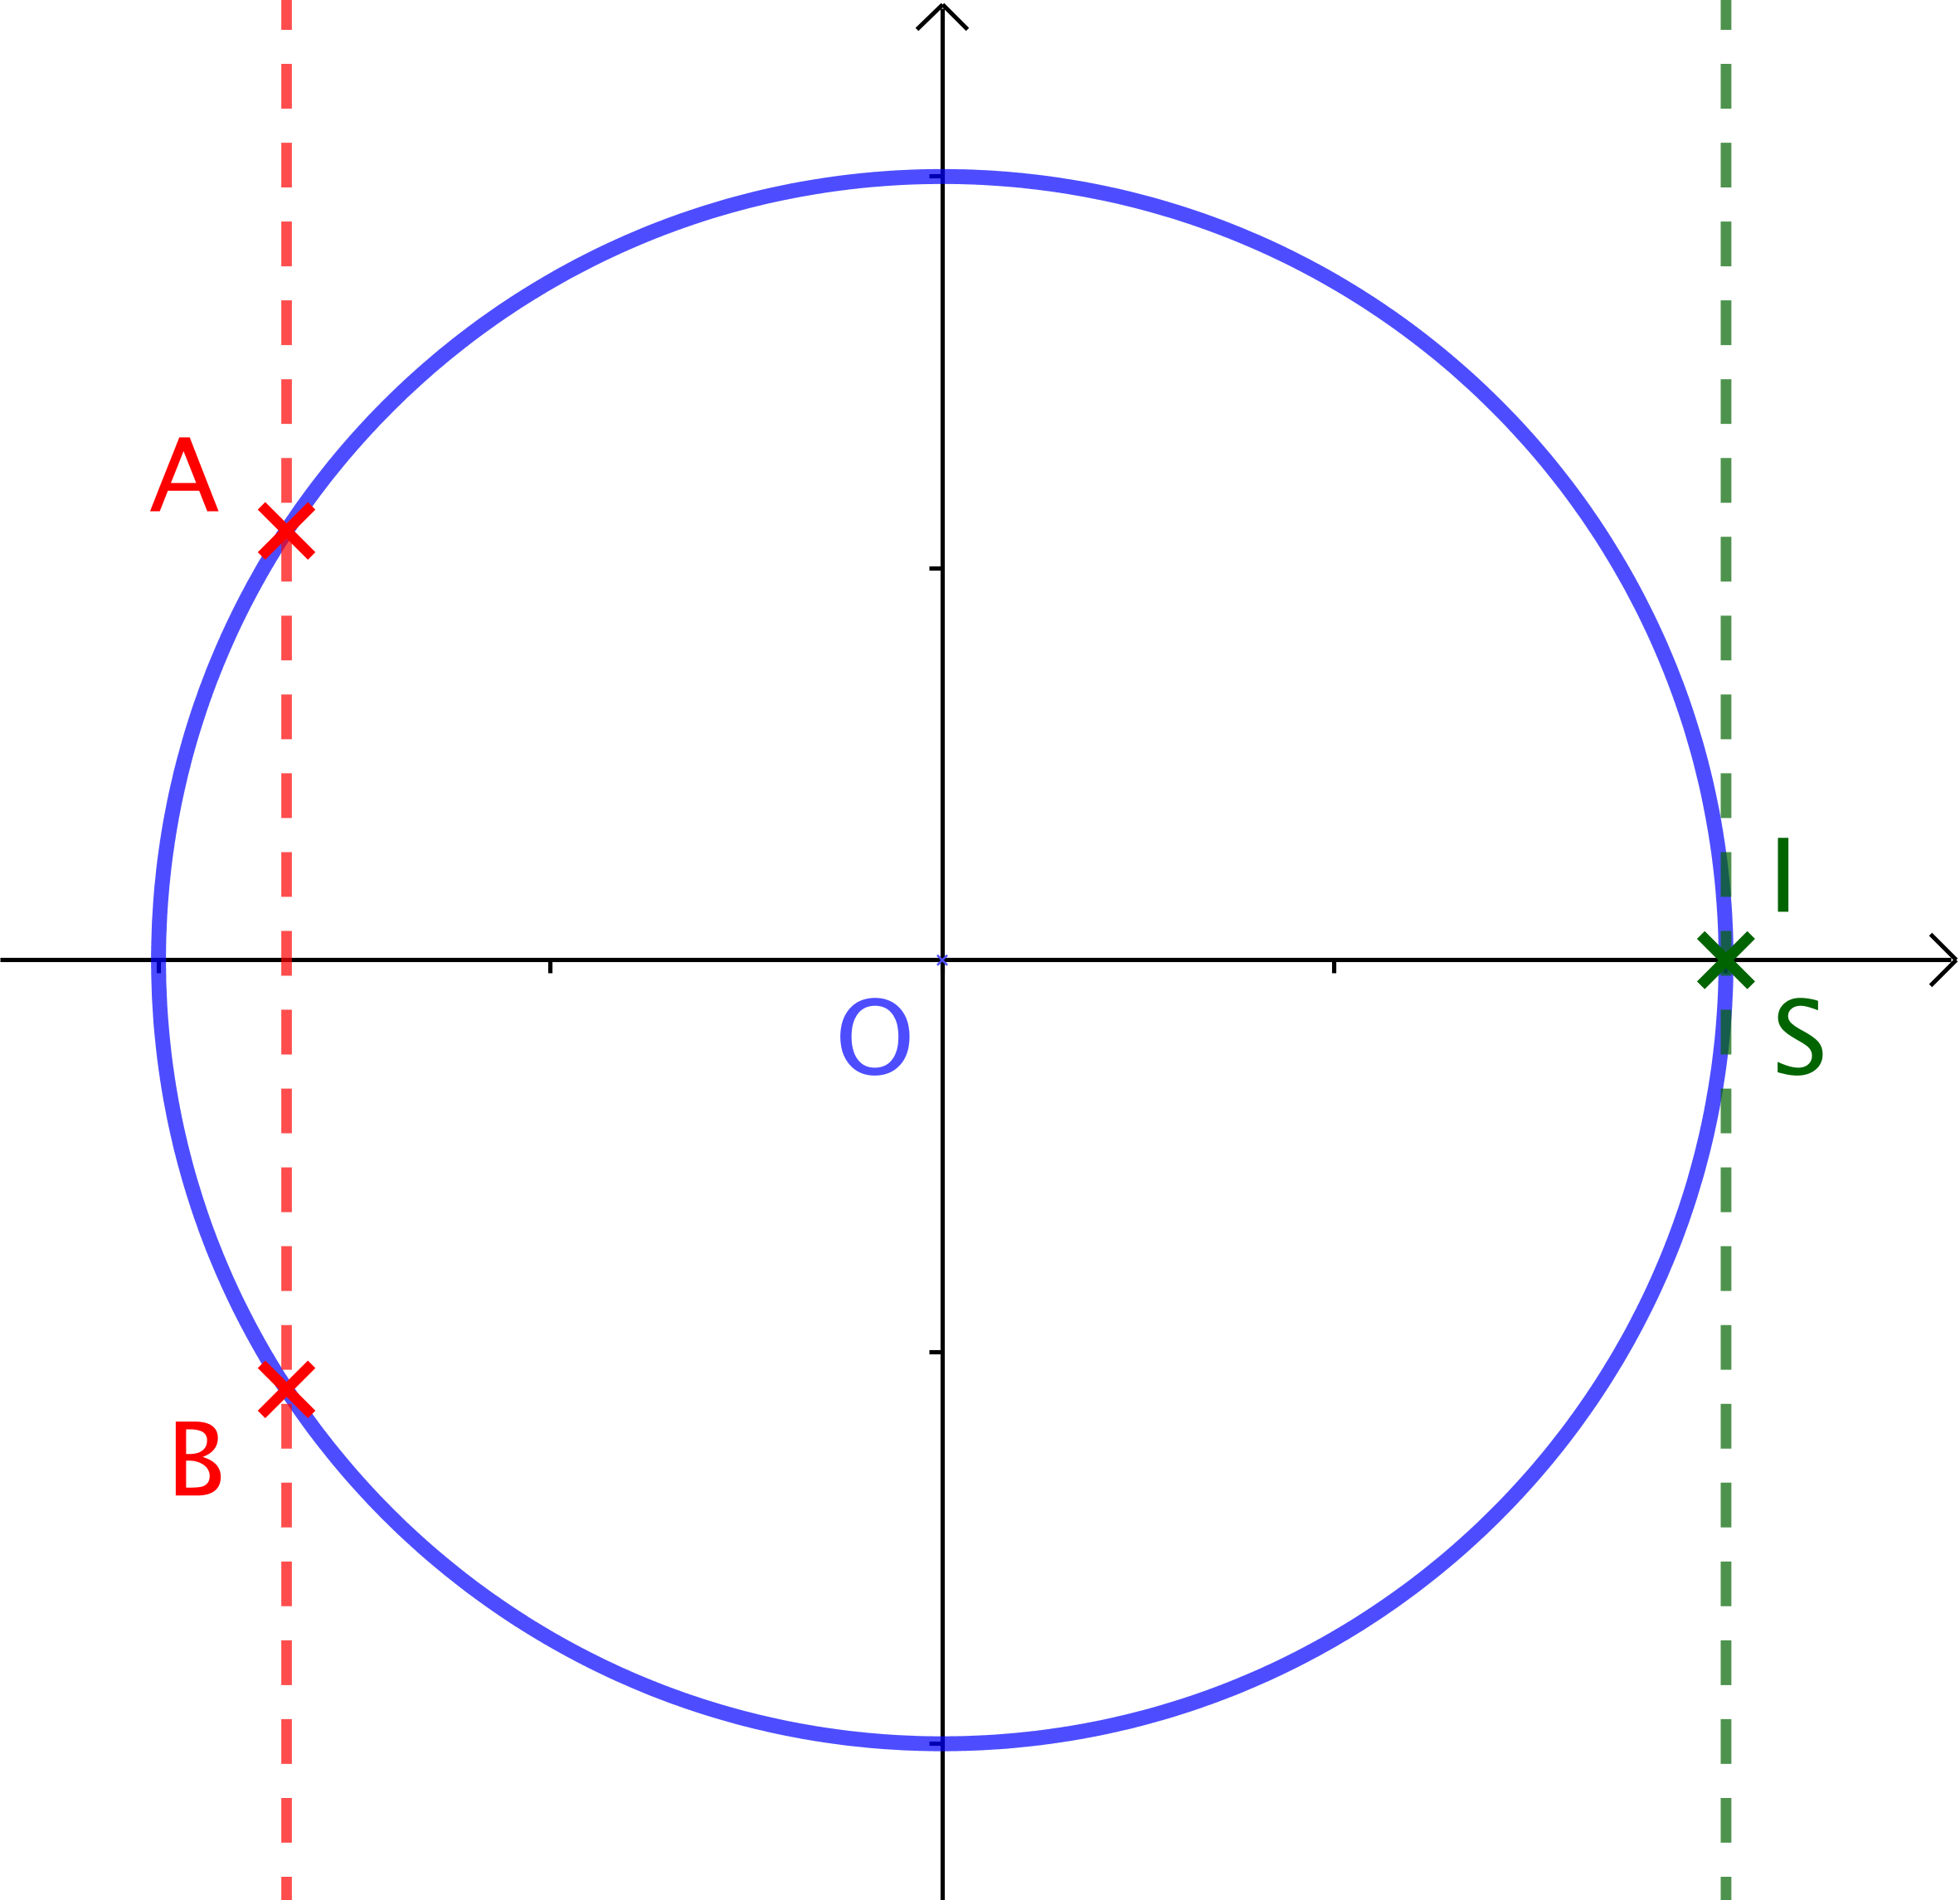
\includegraphics[scale = .75]{addition-on-ellipsis/conjecture/h-sym-with-lines.png}}

	\columnbreak

	\fbox{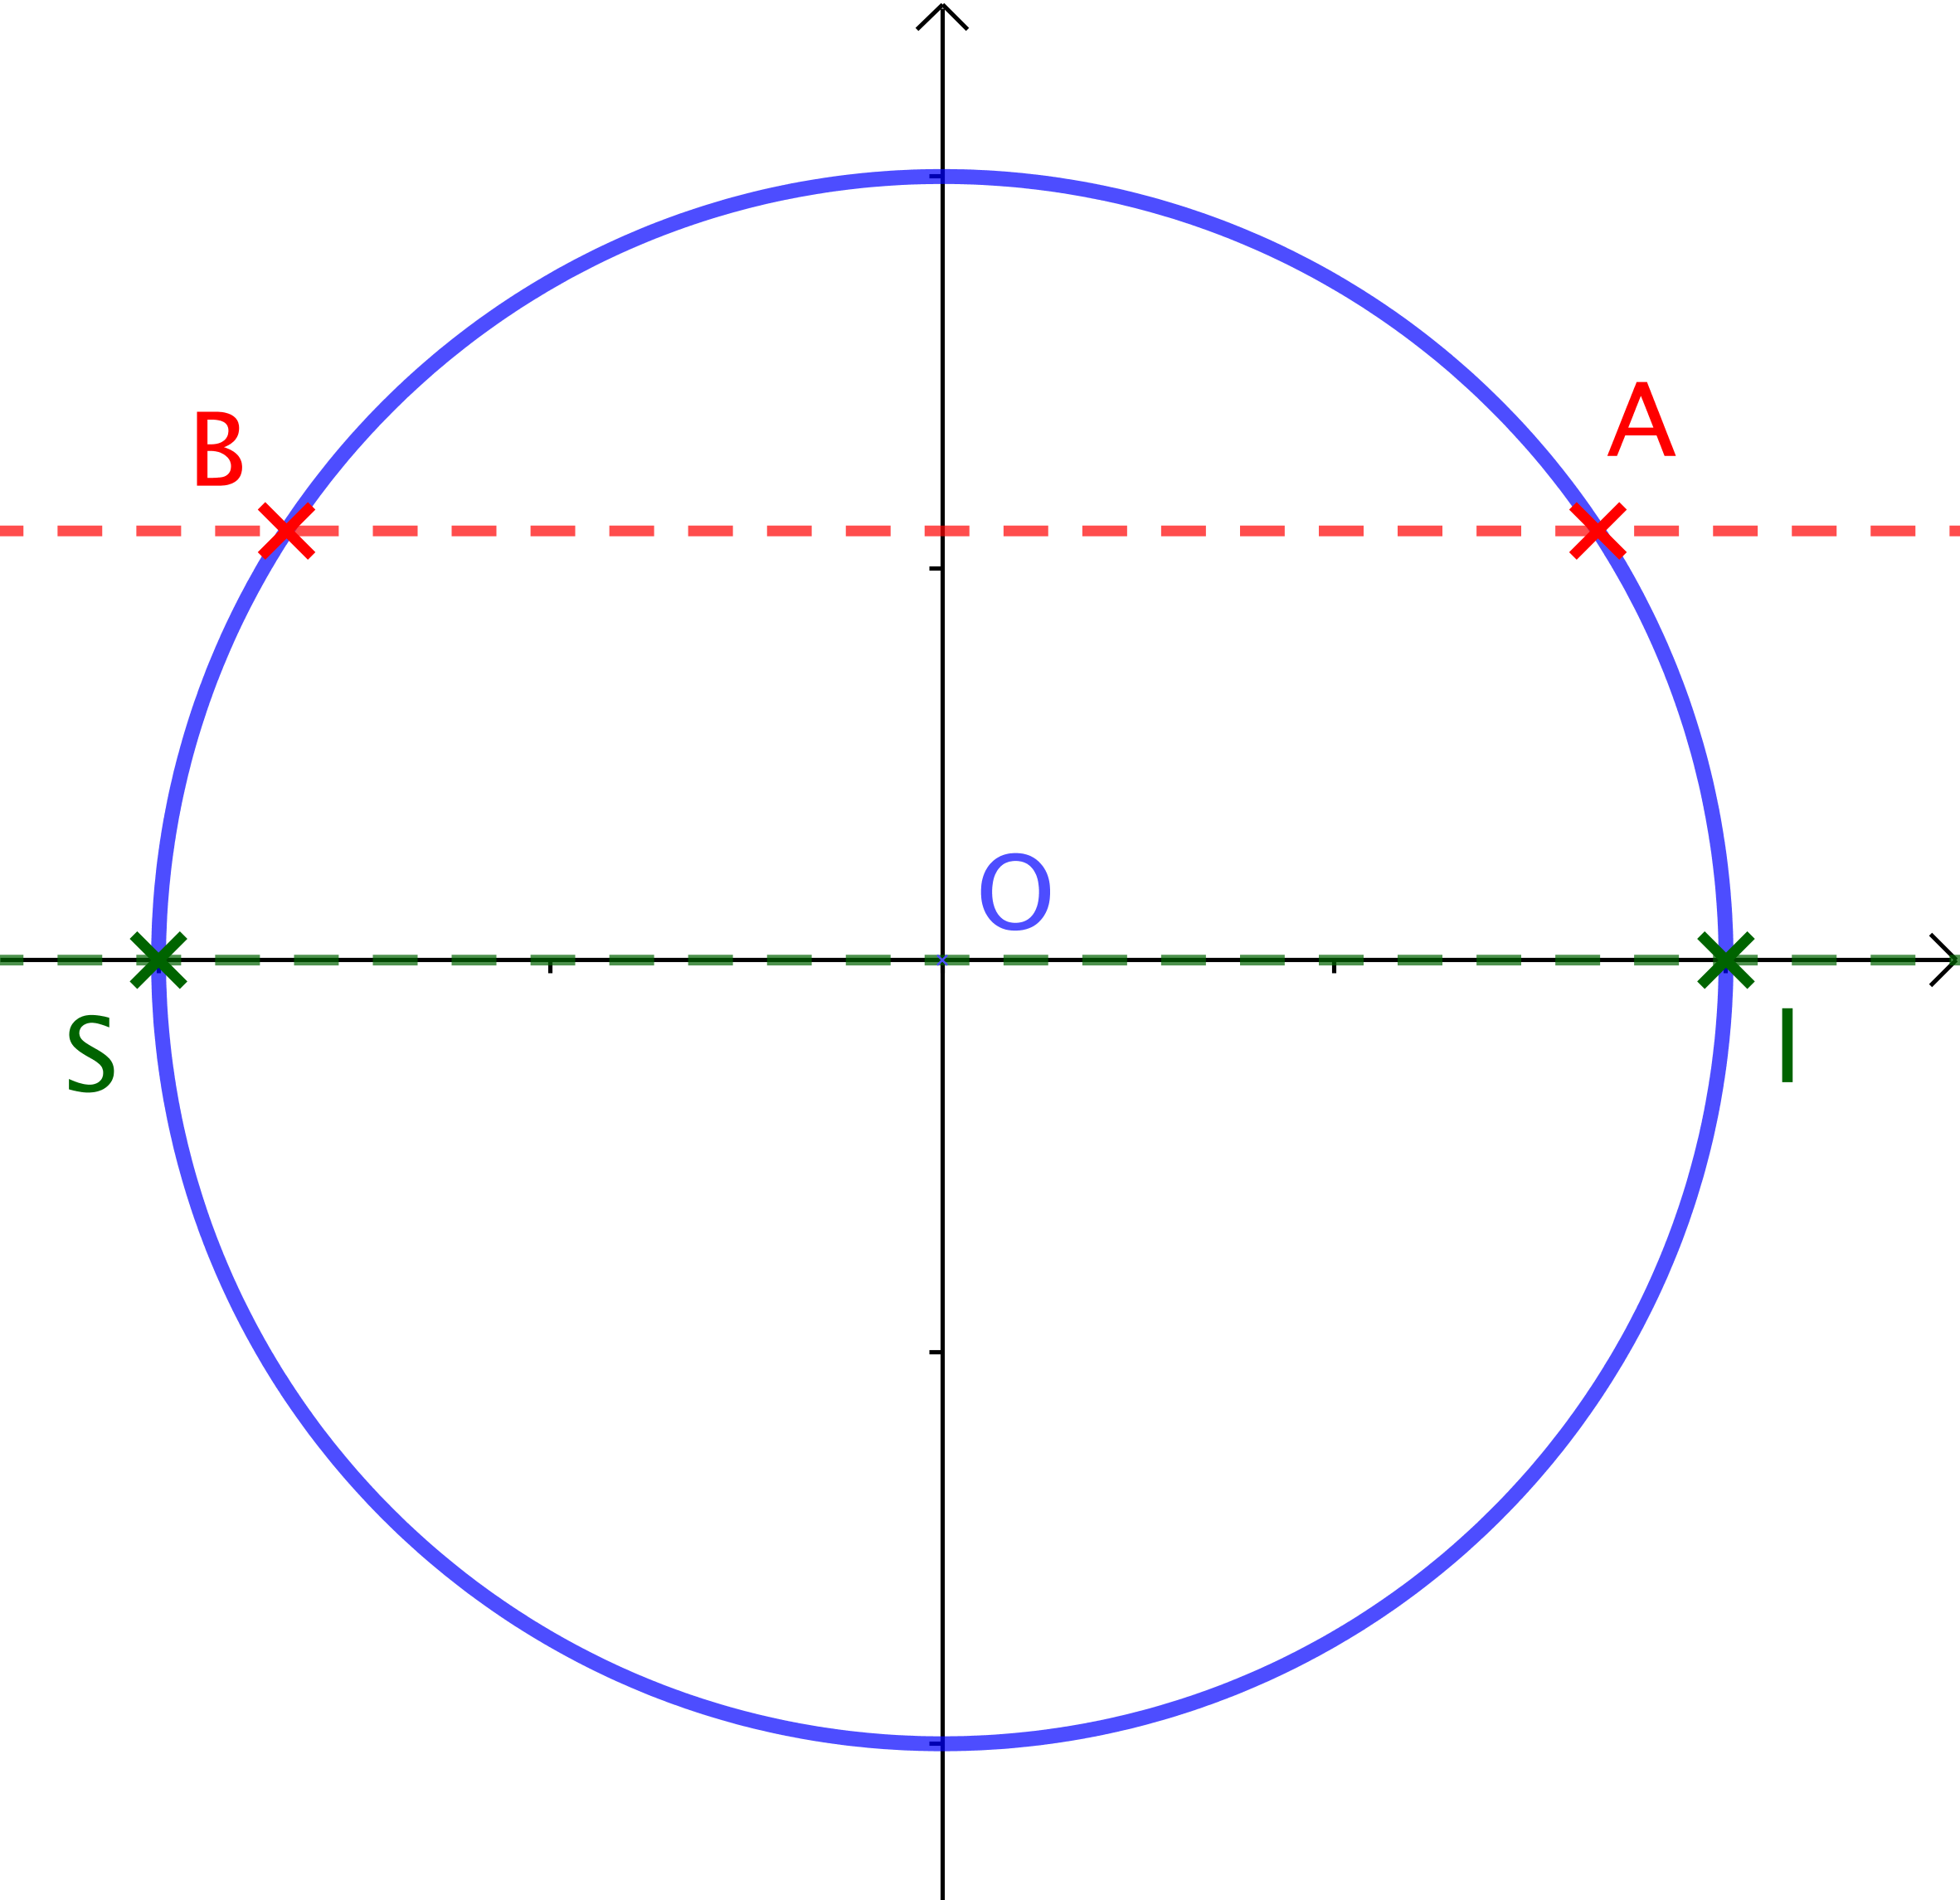
\includegraphics[scale = .75]{addition-on-ellipsis/conjecture/v-sym-with-lines.png}}
\end{multicols}


\medskip

\begin{multicols}{2}
	\center

	\fbox{\includegraphics[scale = .75]{addition-on-ellipsis/conjecture/o-sym-with-lines.png}}

	\columnbreak

	\fbox{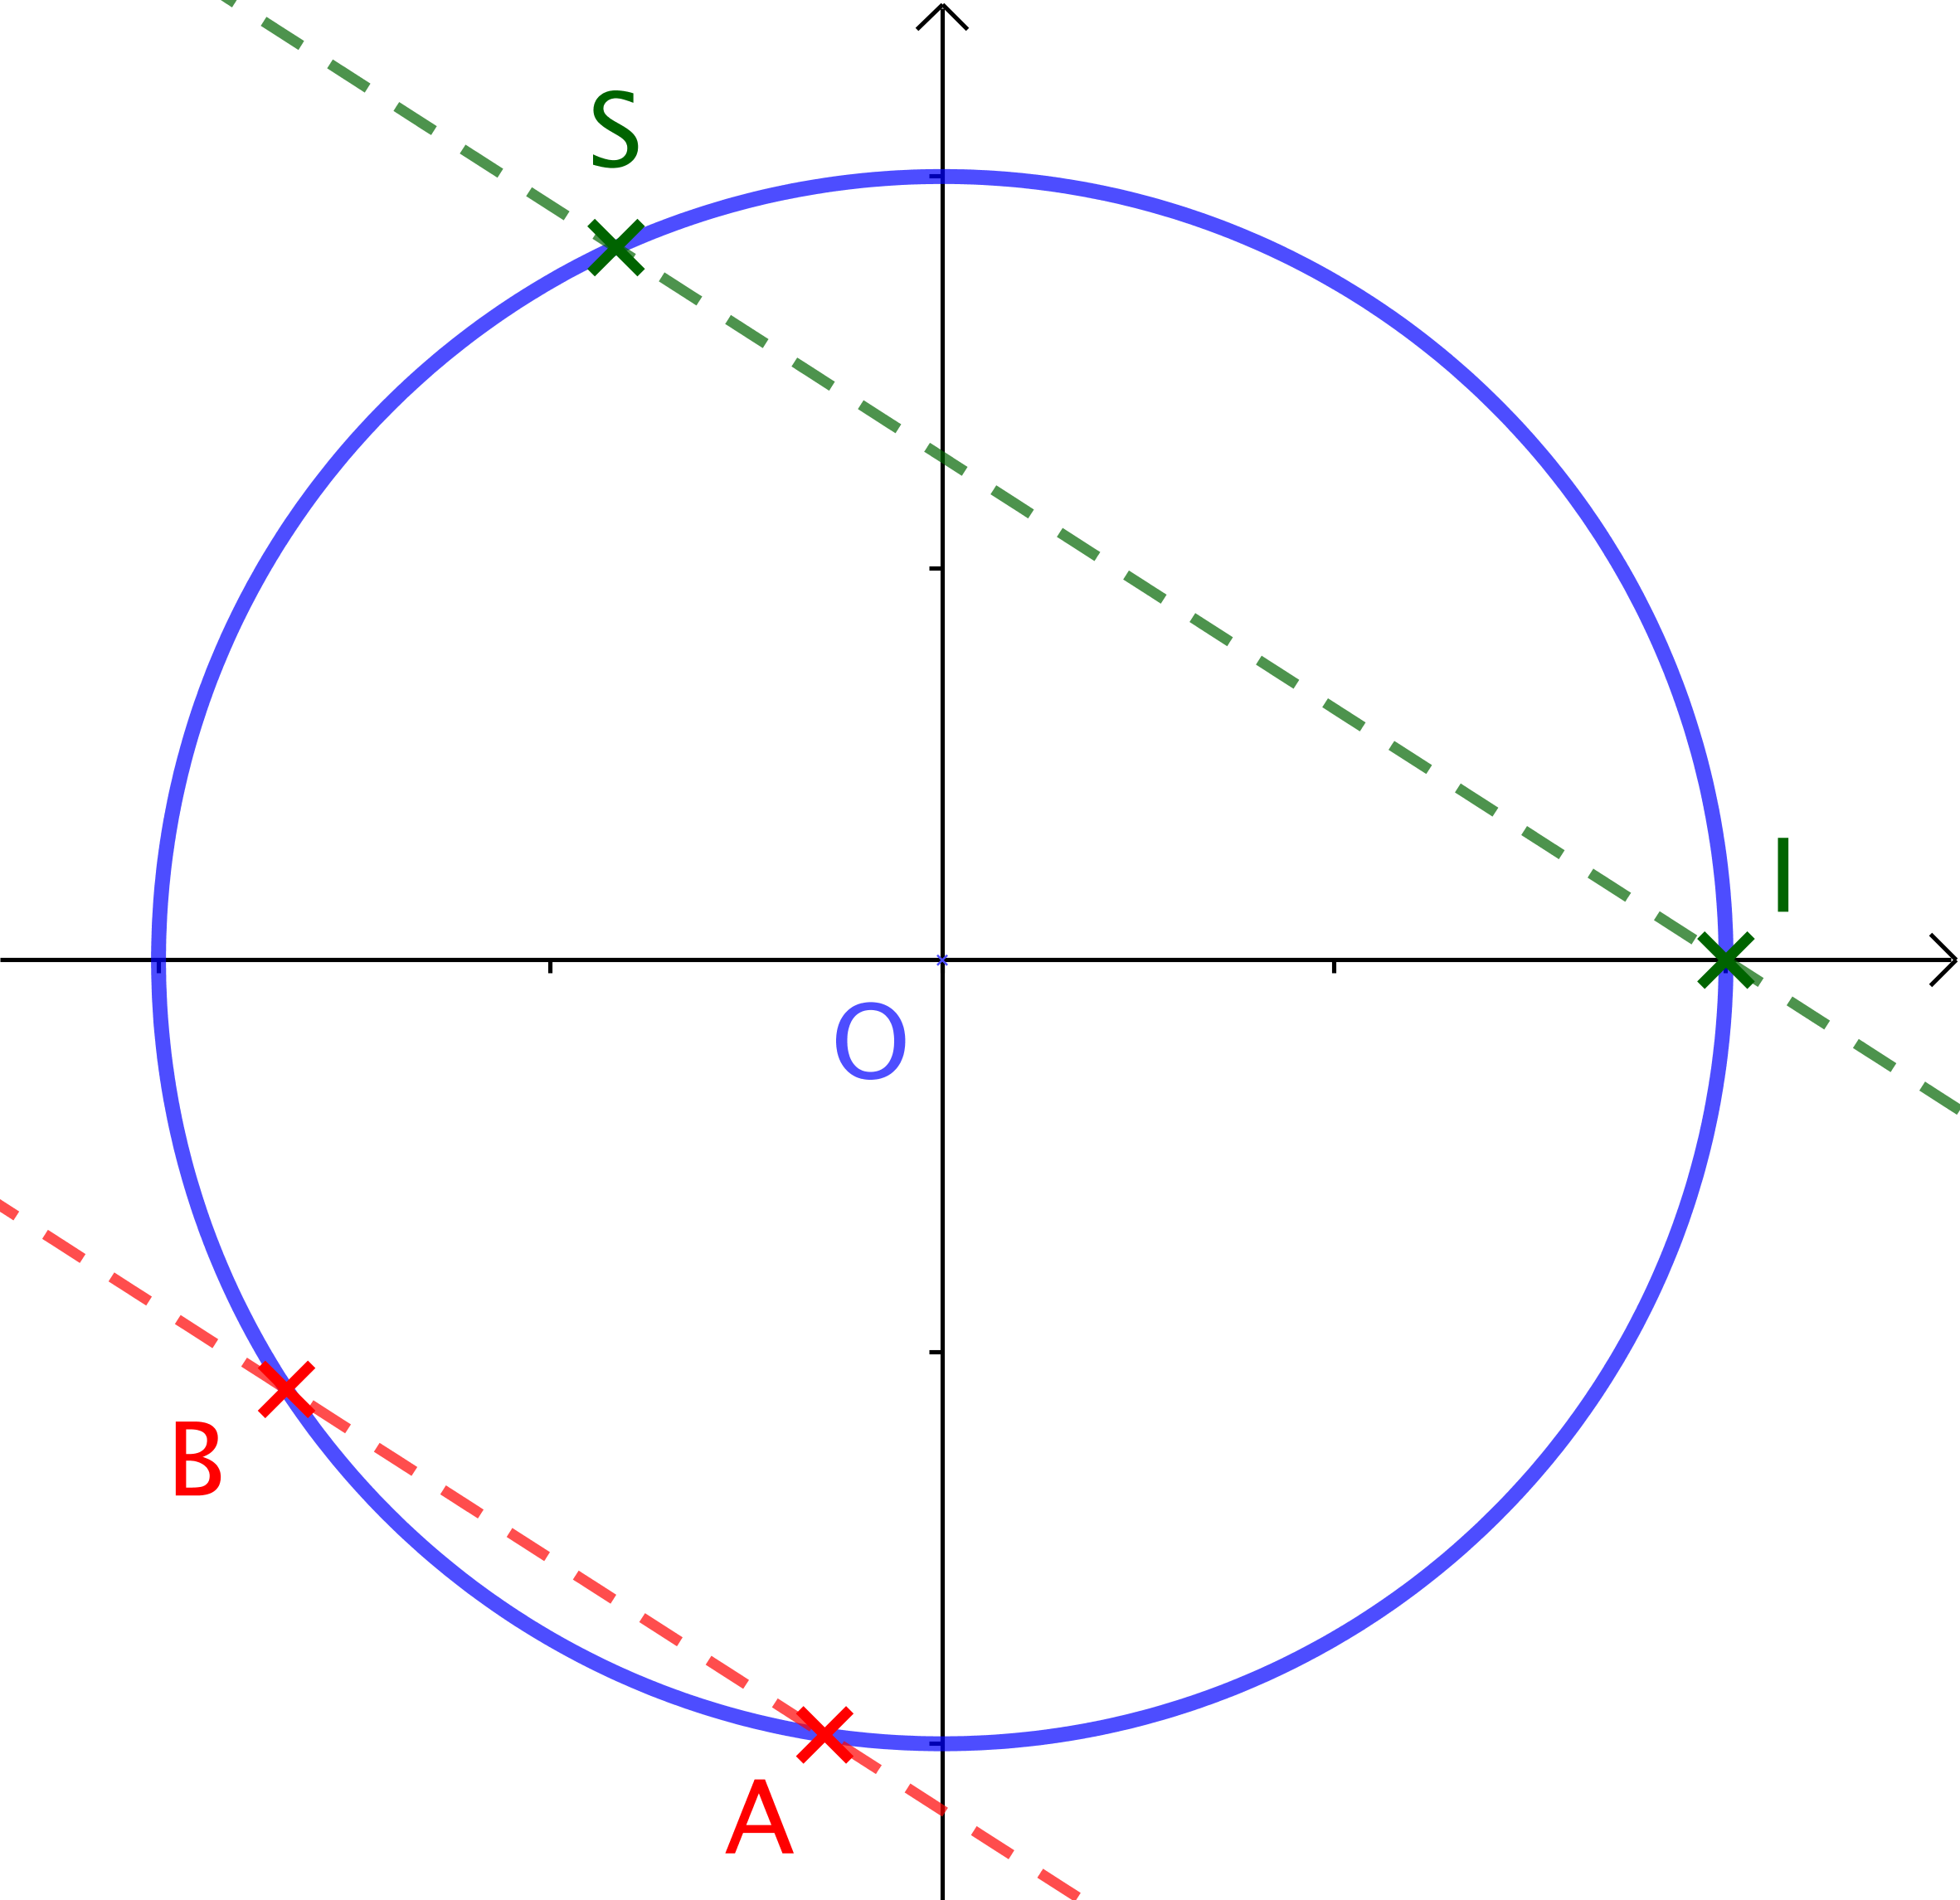
\includegraphics[scale = .75]{addition-on-ellipsis/conjecture/general-with-lines.png}}
\end{multicols}


Il devient évident de conjecturer que le point $S$ se construit géométriquement comme suit.

\begin{enumerate}
	\item \label{point-1} Si $A \neq B$ alors on construit la parallèle à $(AB)$ passant par $I$ . 
	Si cette parallèle n'est pas tangente au cercle alors le point $S$ est le second point d'intersection de cette parallèle avec le cercle, sinon $S = I$ .
	Notons que dans le second cas, c'est à dire si $x_A = x_B$ et $y_A = -y_B$ , alors $S = I$ peut être vu comme un point d'intersection \squote{double}.

	\item Si $A = B$ , on procède comme au point (\ref{point-1}) mais avec la parallèle à la tangente en $A$ au cercle. Intuitivement, cette situation consiste à faire \emph{\og tendre \fg} $A$ vers $B$ 
	\footnote{
		Nous évitons les arguments faisant appel à l'analyse afin de rester dans un cadre géométrique le plus général possible.
	}.
\end{enumerate}


\medskip

Dans ce qui suit nous allons valider cette conjecture de trois façons en allant du plus brutal au plus élégant.

\begin{enumerate}
	\item La 1\iere{} méthode passe assez brutalement via les critères de colinéarité et d'orthogonalité dans un plan.
	
	\item La 2\ieme{} méthode utilise les nombres complexes avec des calculs faciles à mener.
	
	\item La 3\ieme{} méthode, sûrement la plus élégante, est purement géométrique.
\end{enumerate}



\section{Comprendre partiellement\dots}

Essayons de voir, sans chercher à être trop rigoureux, la raison de ce phénomène au travers de deux situations instructives. Ci-après $\setgeo{D}_k \, /\!/ \, \setgeo{d}_k$ pour $k \in \{ 1 \,; 2\}$ et $F$ est le point d'intersection des deux demi-droites.


\medskip


Dans la 1\iere{} situation représentée ci-dessous, nous avons un rayon initial "allant vers $F$" et faisant avec la direction de la demi-droite $\setgeo*{d}{2}$ un angle géométrique $\alpha \in \intervalO{0}{\frac{\pi}{2}}$ , puis au bout de deux rebonds, nous obtenons un rayon "allant vers $F$" avec un angle géométrique de mesure $\alpha + 2\theta$ relativement à la direction de $\setgeo*{d}{2}$.


\medskip


\begin{center}
	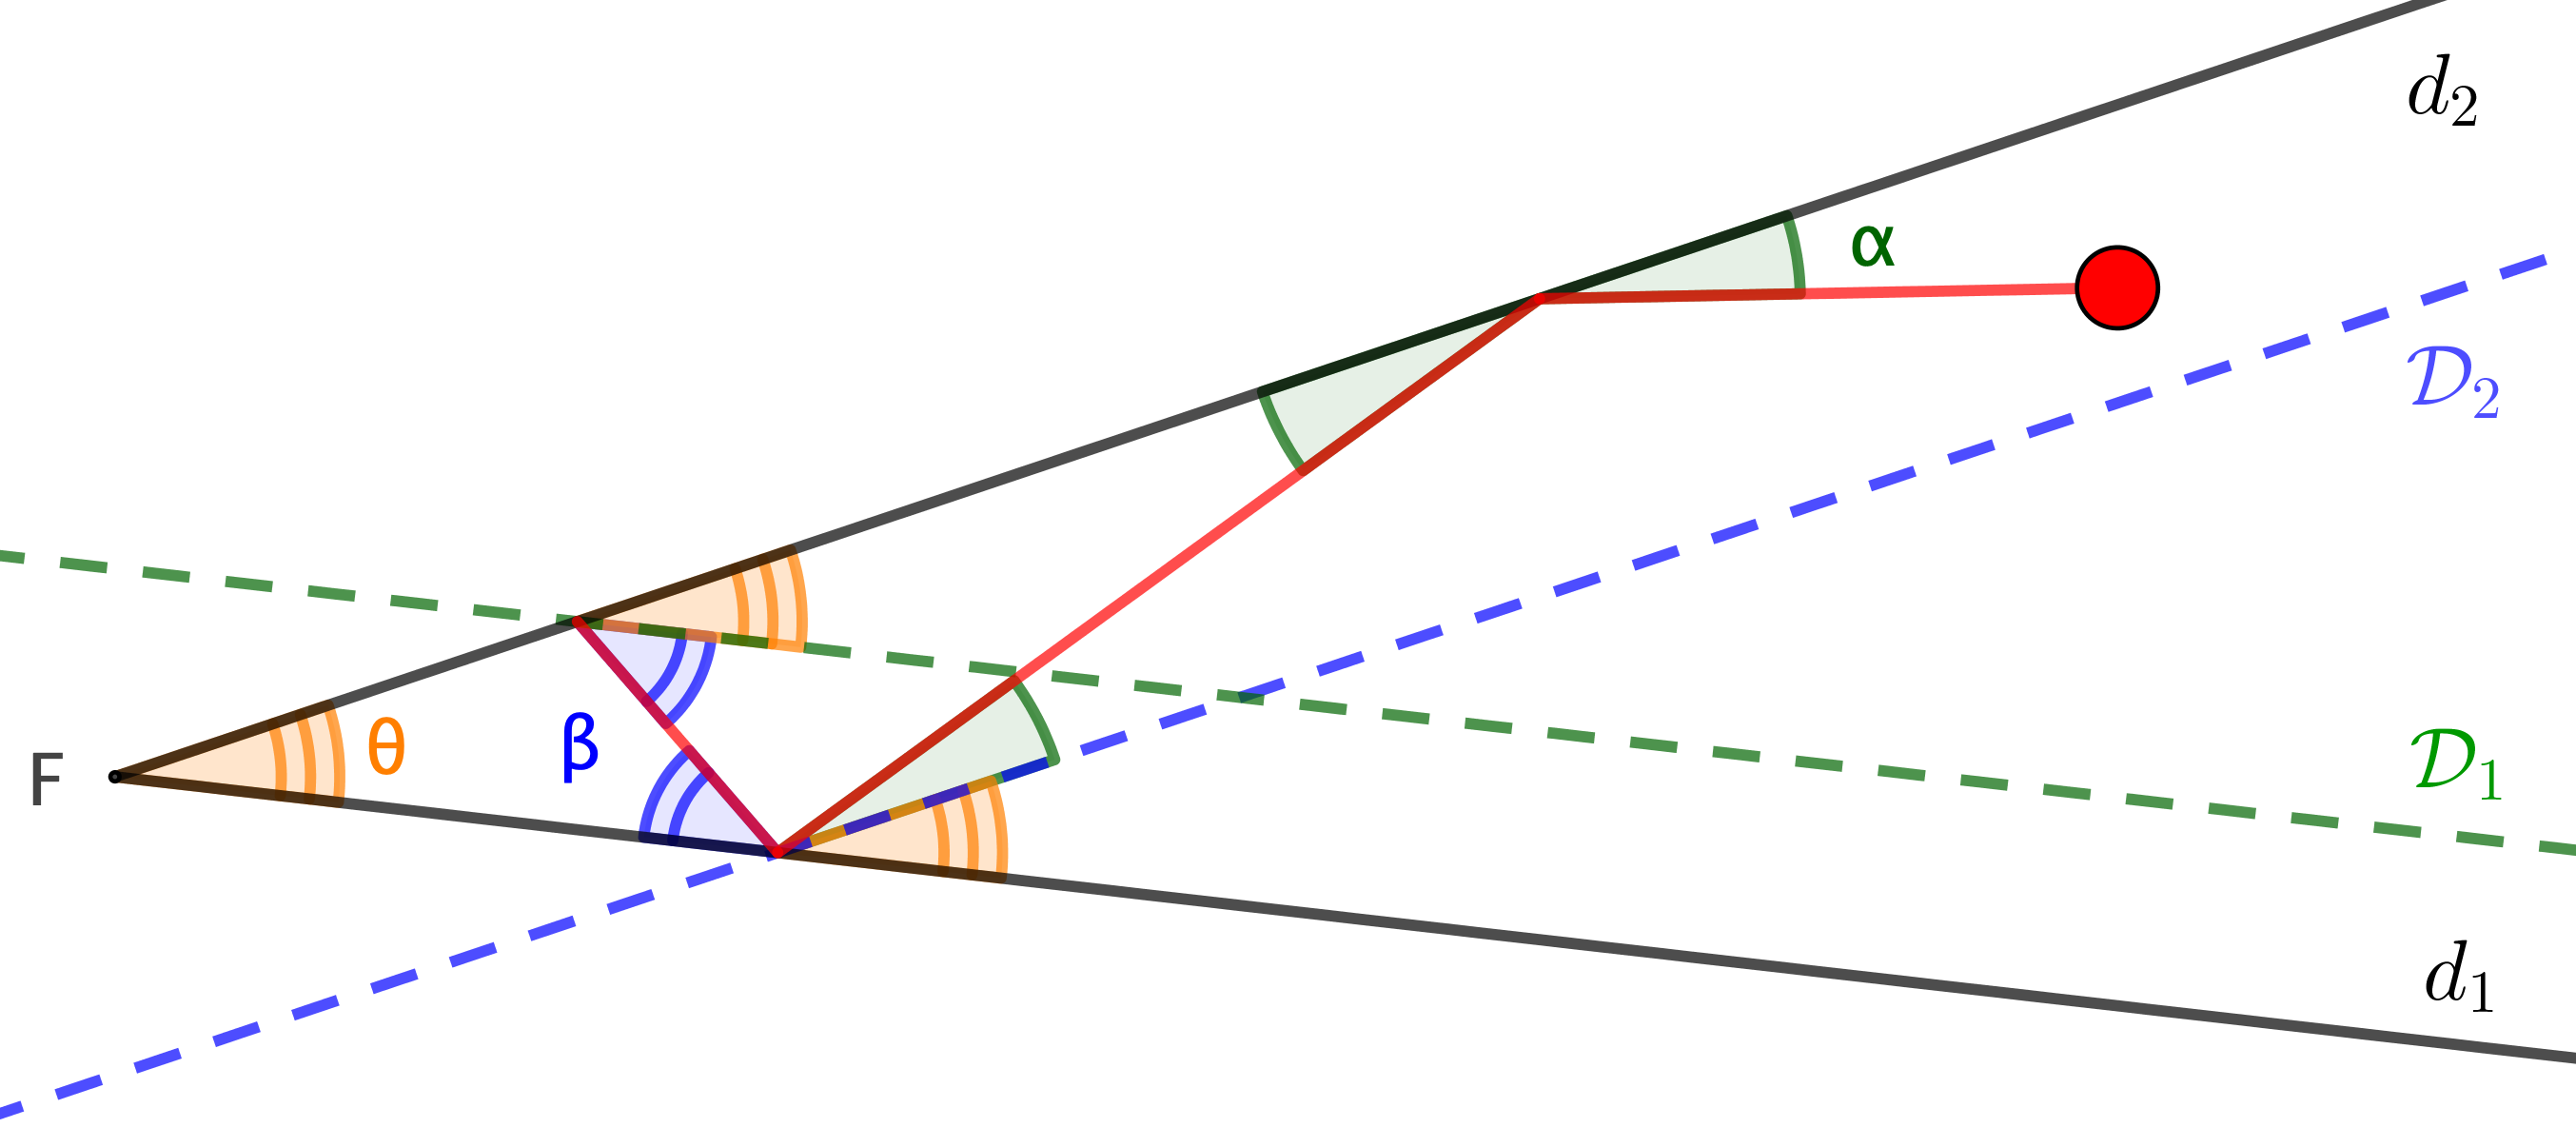
\includegraphics[width=12cm]{basic-math-pool/analysis-1.png}
	
	\itshape\small
	Situation n\textdegree1
	\label{situtation-1}
\end{center}


\medskip


Dans la 2\ieme{} situation ci-après, nous avons un rayon initial "allant à l'opposé de $F$" et faisant  avec la direction de $\setgeo*{d}{2}$ un angle géométrique $\alpha \in \intervalO{0}{\frac{\pi}{2}}$ , puis au bout de deux rebonds, nous obtenons un rayon "allant à l'opposé de $F$" avec un angle géométrique mesurant $\alpha - 2\theta$ relativement à la direction de $\setgeo*{d}{2}$.


\medskip


\begin{center}
	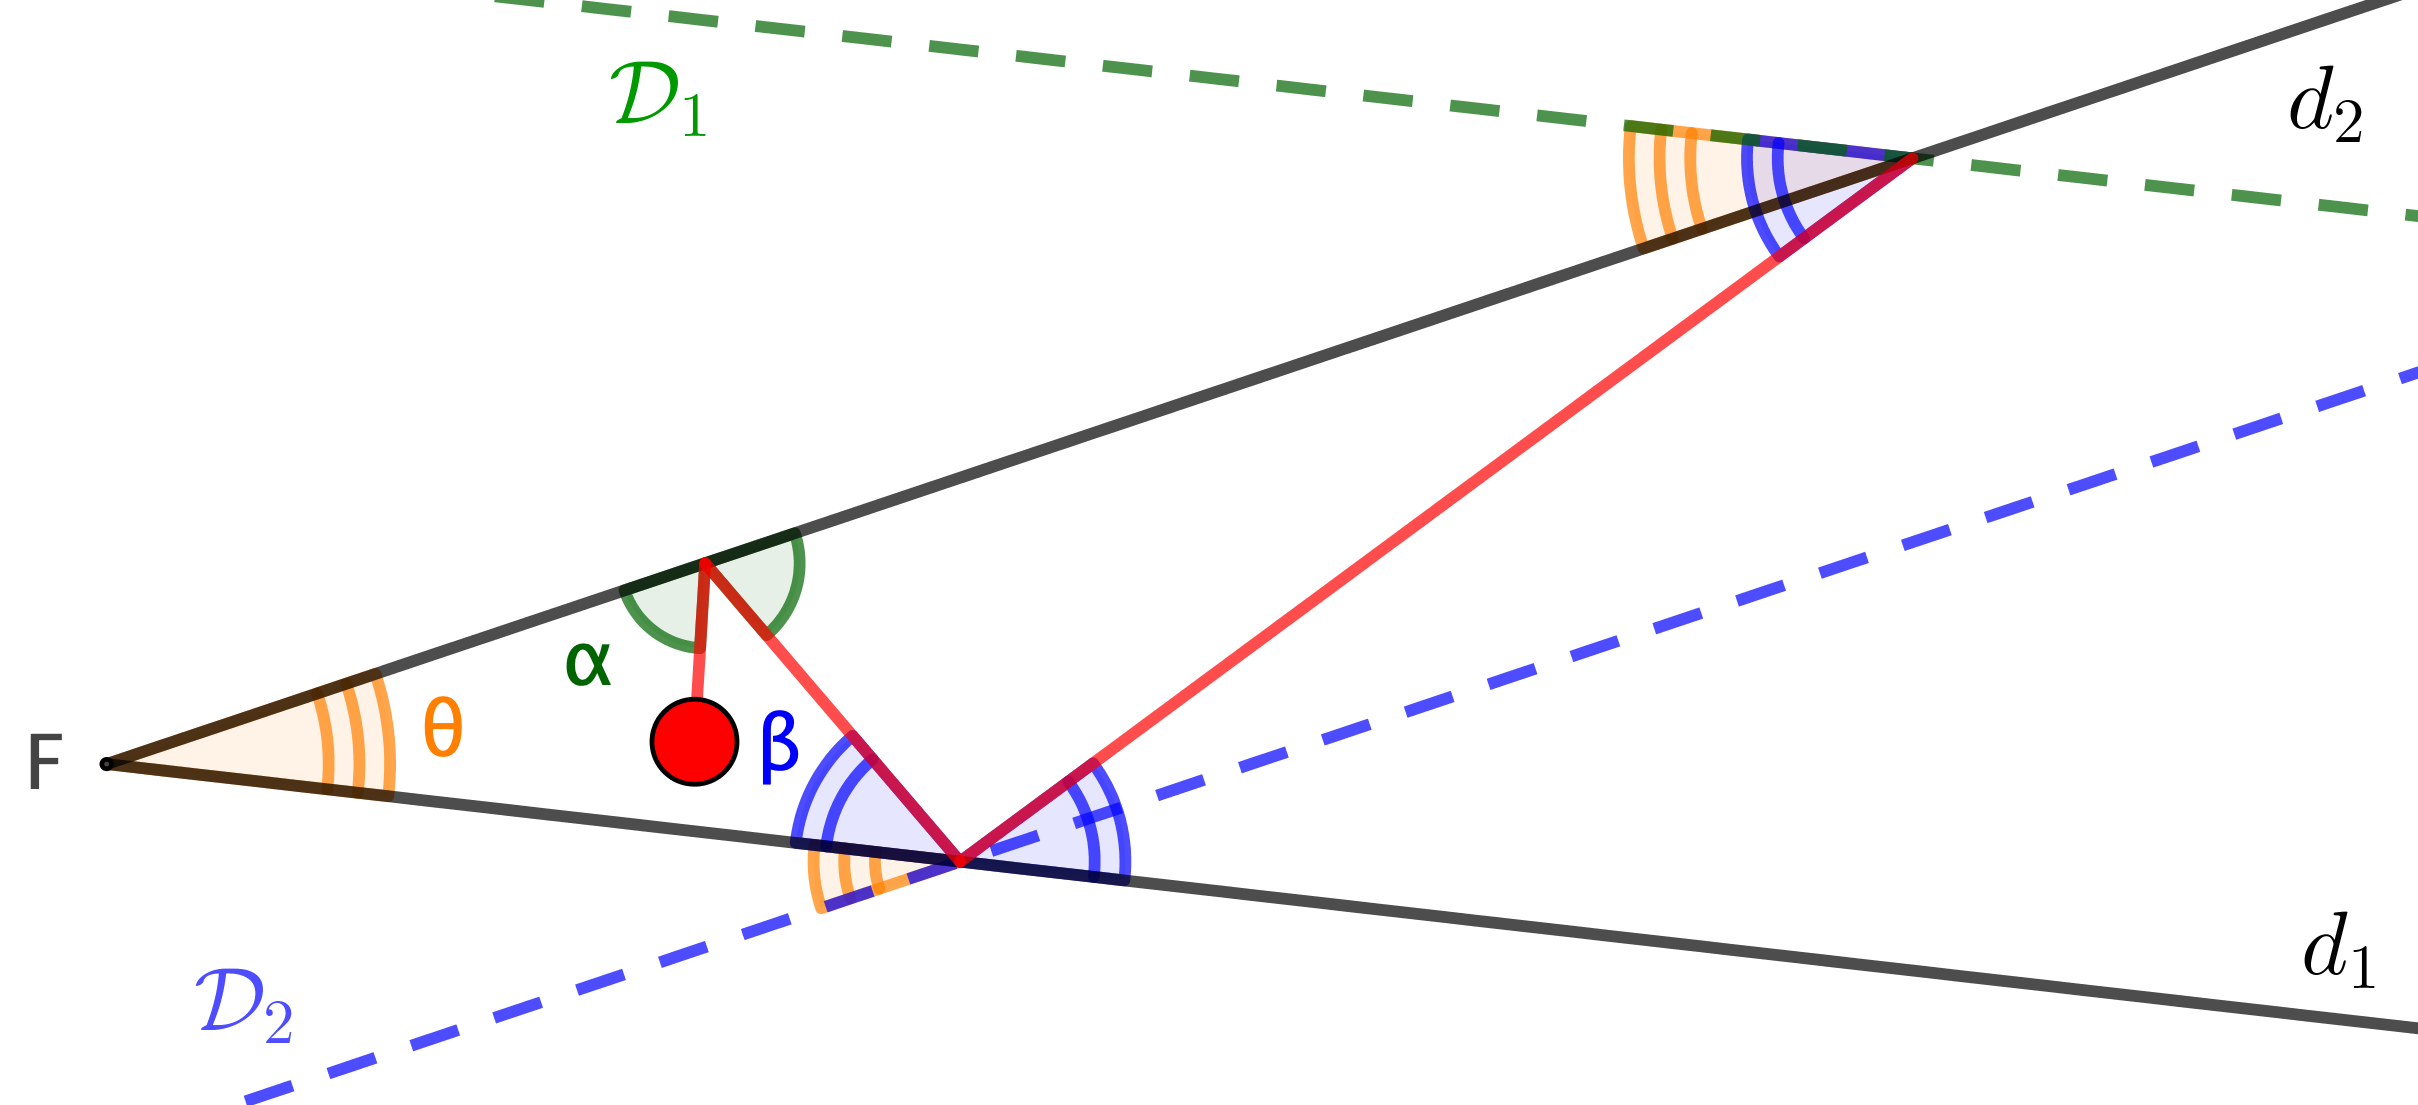
\includegraphics[width=12cm]{basic-math-pool/analysis-2.png}
	
	\itshape\small
	Situation n\textdegree2
	\label{situtation-2}
\end{center}


\medskip

Imaginons que notre bille soit d'abord confrontée à la situation n\textdegree1. Au bout de deux rebonds, l'angle relativement à $\setgeo*{d}{2}$ passe de $\alpha_0 = \alpha$ à $\alpha_1 = \alpha + 2 \theta$. Une suite successive de situations n\textdegree1 va donc faire augmenter l'angle par rapport à la direction de $\setgeo*{d}{2}$. Il arrivera donc un moment où la situation n\textdegree2 arrivera, excepté si l'on obtient un rebond perpendiculaire à $\setgeo*{d}{2}$. Nous ignorons ici ce cas qui sera géré dans notre démonstration.

Une fois que la situation n\textdegree2 se présente, nous avons des angles de plus en plus petit relativement à $\setgeo*{d}{2}$ jusqu'à arriver au dernier rebond possible après lequel la bille s'éloignera indéfiniment. Voilà une explication partielle du phénomène.


\section{Notations pour la suite}

Tous les angles sont orientés et confondus abusivement avec leur mesure principale.
\begin{enumerate}
	\item $\setgeo*{d}{1}$ et $\setgeo*{d}{2}$ sont deux demi-droites d'origine $F$ et telles que $\theta = \langle \setgeo*{d}{1} \,; \setgeo*{d}{2} \rangle \in \intervalO{0}{\dfrac{\pi}{2}}$ .

	\item $S$, le point de départ, est tel que $S \notin \setgeo*{d}{1} \cup \setgeo*{d}{2}$ et $\tau = \langle \setgeo*{d}{1} \,; [FS) \rangle \in \intervalO{0}{\theta}$ .
	
	\item Pour tout point $M$ du plan, nous noterons $H_M$ sont projeté orthogonal sur $\setgeo*{d}{2}$.
	
	\item Pour tout point $M$ qui est sur le trajet de la bille, mais pas sur $\setgeo*{d}{2}$, si $D_M$ est un point tel que $\vect{MD_M}$ indique la direction et le sens du trajet "sortant" de $M$, nous notons $\sigma_M = \langle \vect{MH_M} \,; \vect{MD_M} \rangle$.
\end{enumerate}


\medskip


\begin{center}
	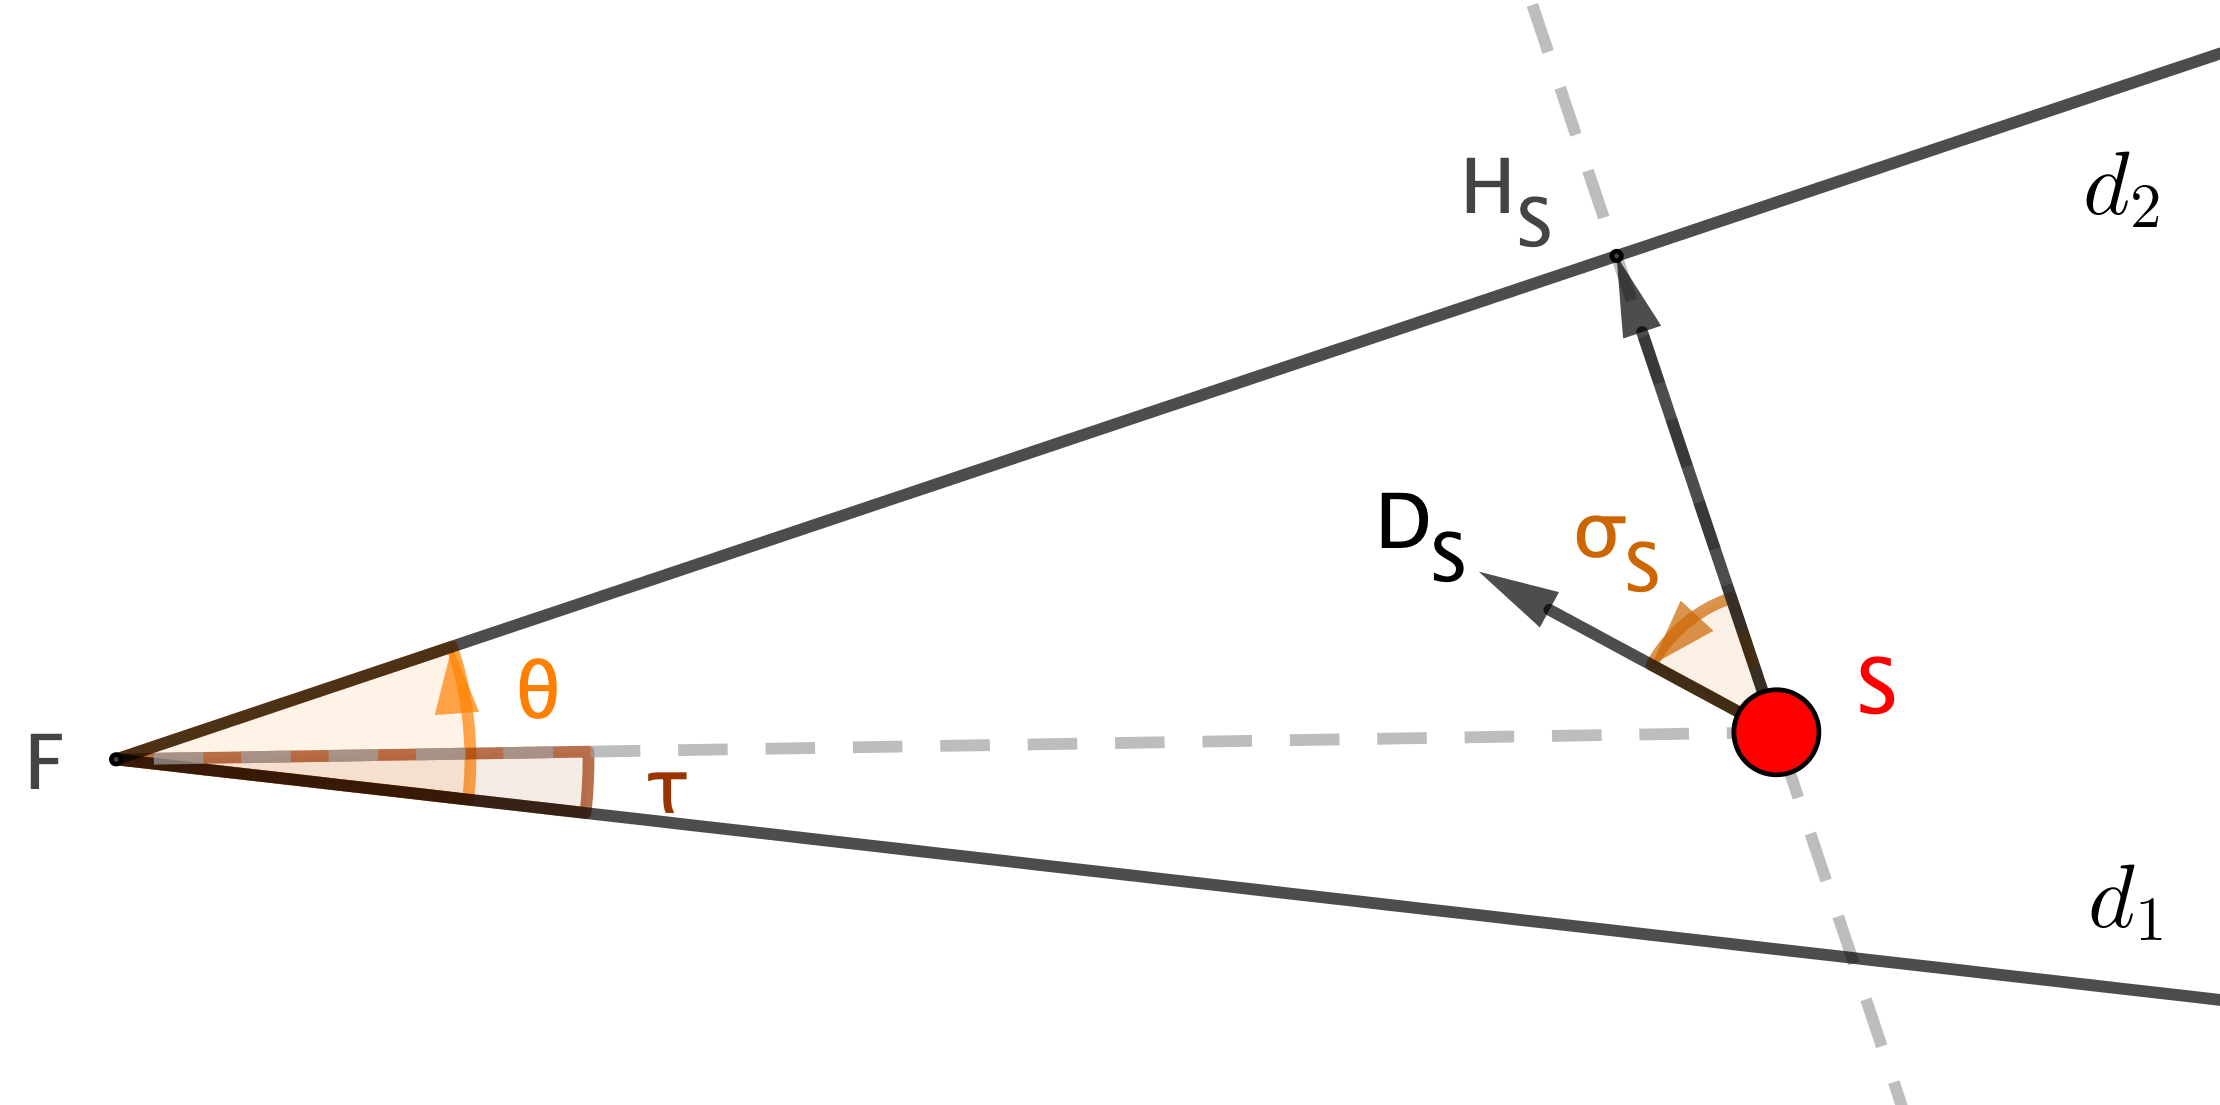
\includegraphics[width=12cm]{basic-math-pool/proof-notations.png}
	
	\itshape\small
	Notations pour la suite
\end{center}





\section{Où se fait le 1\ier{} rebond ?}
\label{1st-bounce}

\begin{fact}
	Nous avons les cas initiaux suivants.
	
	\begin{itemize}[label = \small\textbullet]
		\item Il n'y a aucun rebond si et seulement si $\sigma_S \in \intervalC{- \dfrac{\pi}{2} - \theta}{- \dfrac{\pi}{2}}$.
		
		\item La bille va directement vers $F$ si et seulement si $\sigma_S = \dfrac{\pi}{2} - \theta + \tau$.

		\item Le 1\ier{} rebond se fait sur $\setgeo*{d}{1}$ si et seulement si $\sigma_S \in \intervalOC{\dfrac{\pi}{2} - \theta + \tau}{\pi} \cup \intervalO{- \pi}{- \dfrac{\pi}{2} - \theta}$.

		\item Le 1\ier{} rebond se fait sur $\setgeo*{d}{2}$ si et seulement si $\sigma_S \in \intervalO{- \dfrac{\pi}{2}}{\dfrac{\pi}{2} - \theta + \tau}$.
	\end{itemize}

\end{fact}

\begin{proof}
	Tout est contenu dans les deux dessins suivants où $\setgeo*{D}{k} \, /\!/ \, \setgeo*{d}{k}$ pour $k \in \{ 1 \,; 2\}$.

	\medskip

	\begin{center}
		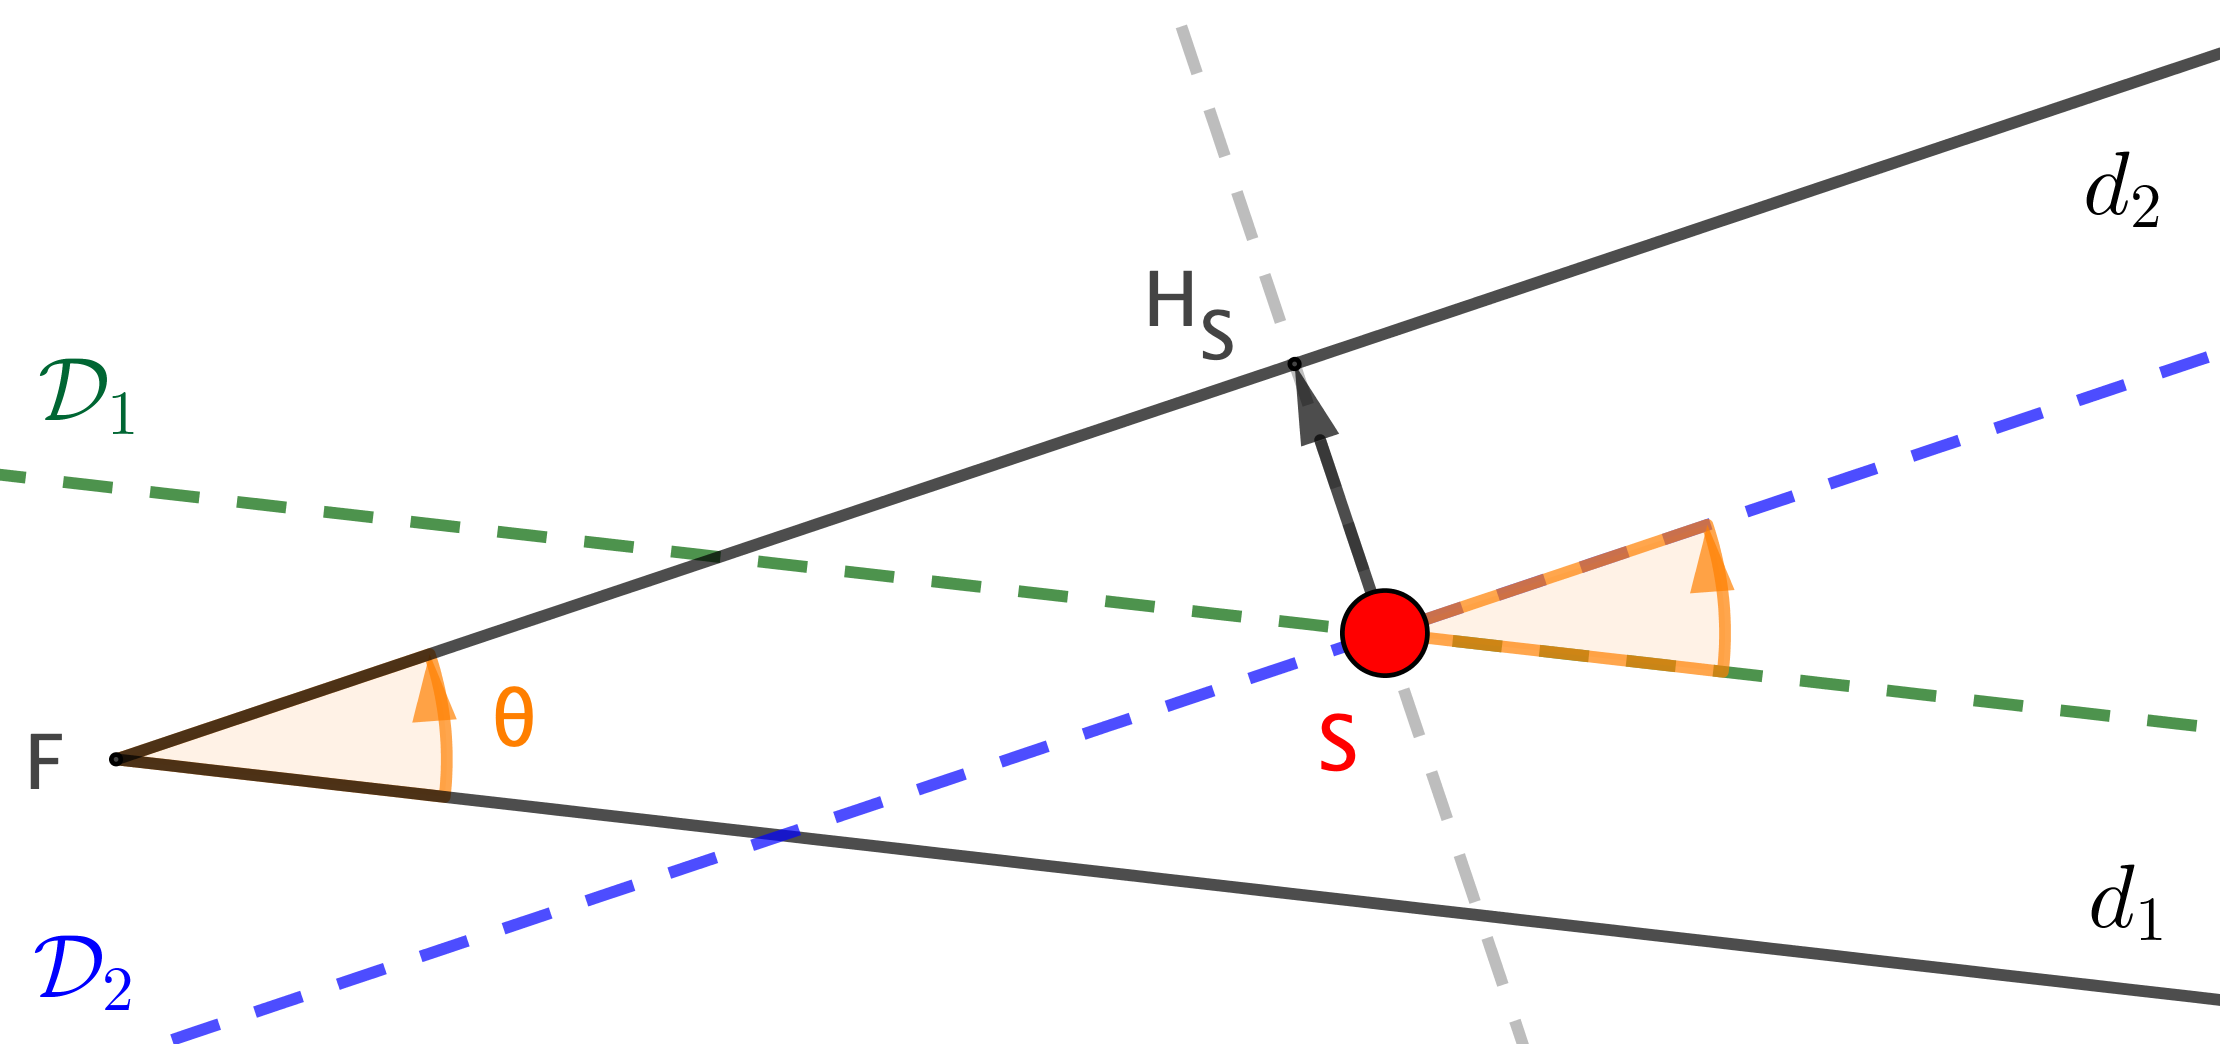
\includegraphics[width=12cm]{basic-math-pool/proof-no-bounce.png}

		\itshape\small
		Aucun 1\ier{} rebond
	\end{center}

	\medskip

	\begin{center}
		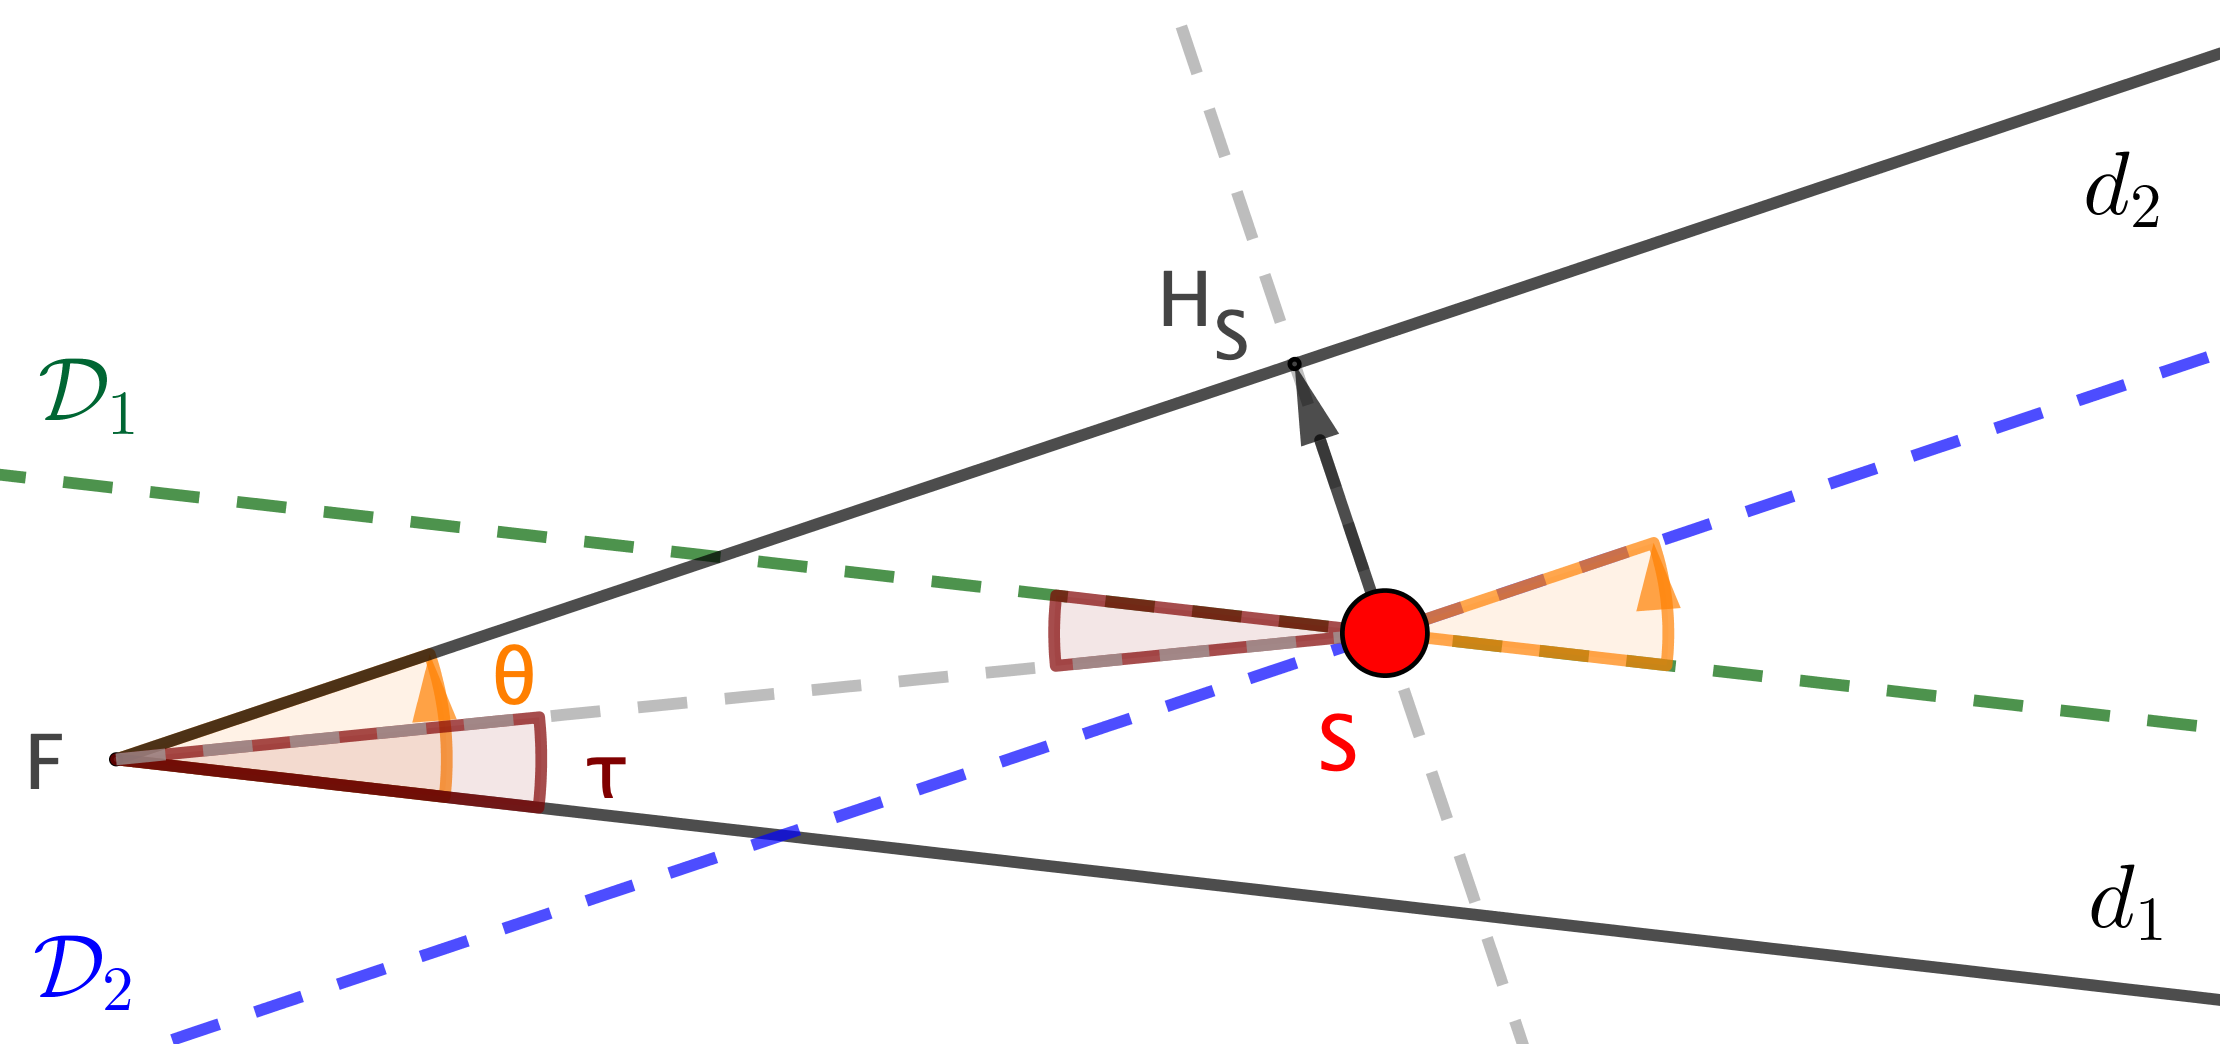
\includegraphics[width=12cm]{basic-math-pool/proof-1st-bounce-somewhere.png}

		\itshape\small
		Les autres cas
	\end{center}
\end{proof}


Il nous reste juste à traiter les cas d'un 1\ier{} rebond se faisant sur $\setgeo*{d}{1}$ et $\setgeo*{d}{2}$ respectivement.

\begin{tcolorbox}
	\centering\itshape
	
	En fait, nous n'avons besoin de traiter que la situation d'un 1\ier{} rebond sur $\setgeo*{d}{2}$.
\end{tcolorbox}

En effet, une fois ceci étudié, l'autre cas s'obtiendra avec le même type de raisonnement excepté que l'on projettera $S$ sur $\setgeo*{d}{1}$ au lieu de $\setgeo*{d}{2}$.



\section{Quand le 1\ier{} rebond se fait "vers le haut"}

\begin{fact} \label{ortho-rebond}
	Supposons que $\sigma_S = 0$.
	
	\medskip
	
	Notant $M$ l'intersection de $(SH_S)$ avec $\setgeo*{d}{1}$, nous avons que $M$ est sur le trajet de la bille avec $\sigma_M < 0$
	\footnote{
		On pourrait avoir un résultat plus fin mais ceci ne nous serait inutile pour la suite.
	}.
\end{fact}

\begin{proof}
	Évident grâce au dessin précédent.
\end{proof}


\medskip


\begin{fact} \label{deux-rebonds-vers-F}
	Supposons que $\sigma_S \in \intervalO{0}{\dfrac{\pi}{2} - \theta + \tau}$.
	
	\medskip
	
	Il existe un point $M$ sur le trajet de la bille, mais pas sur $\setgeo*{d}{1}$, tel que $\sigma_M  < 0$.
\end{fact}

\begin{proof}
	Au bout de deux rebonds, nous avons trois situations possibles dont les deux premières ci-après ne nécessitent aucune explication.
	
	
	\medskip
	
	\begin{center}
		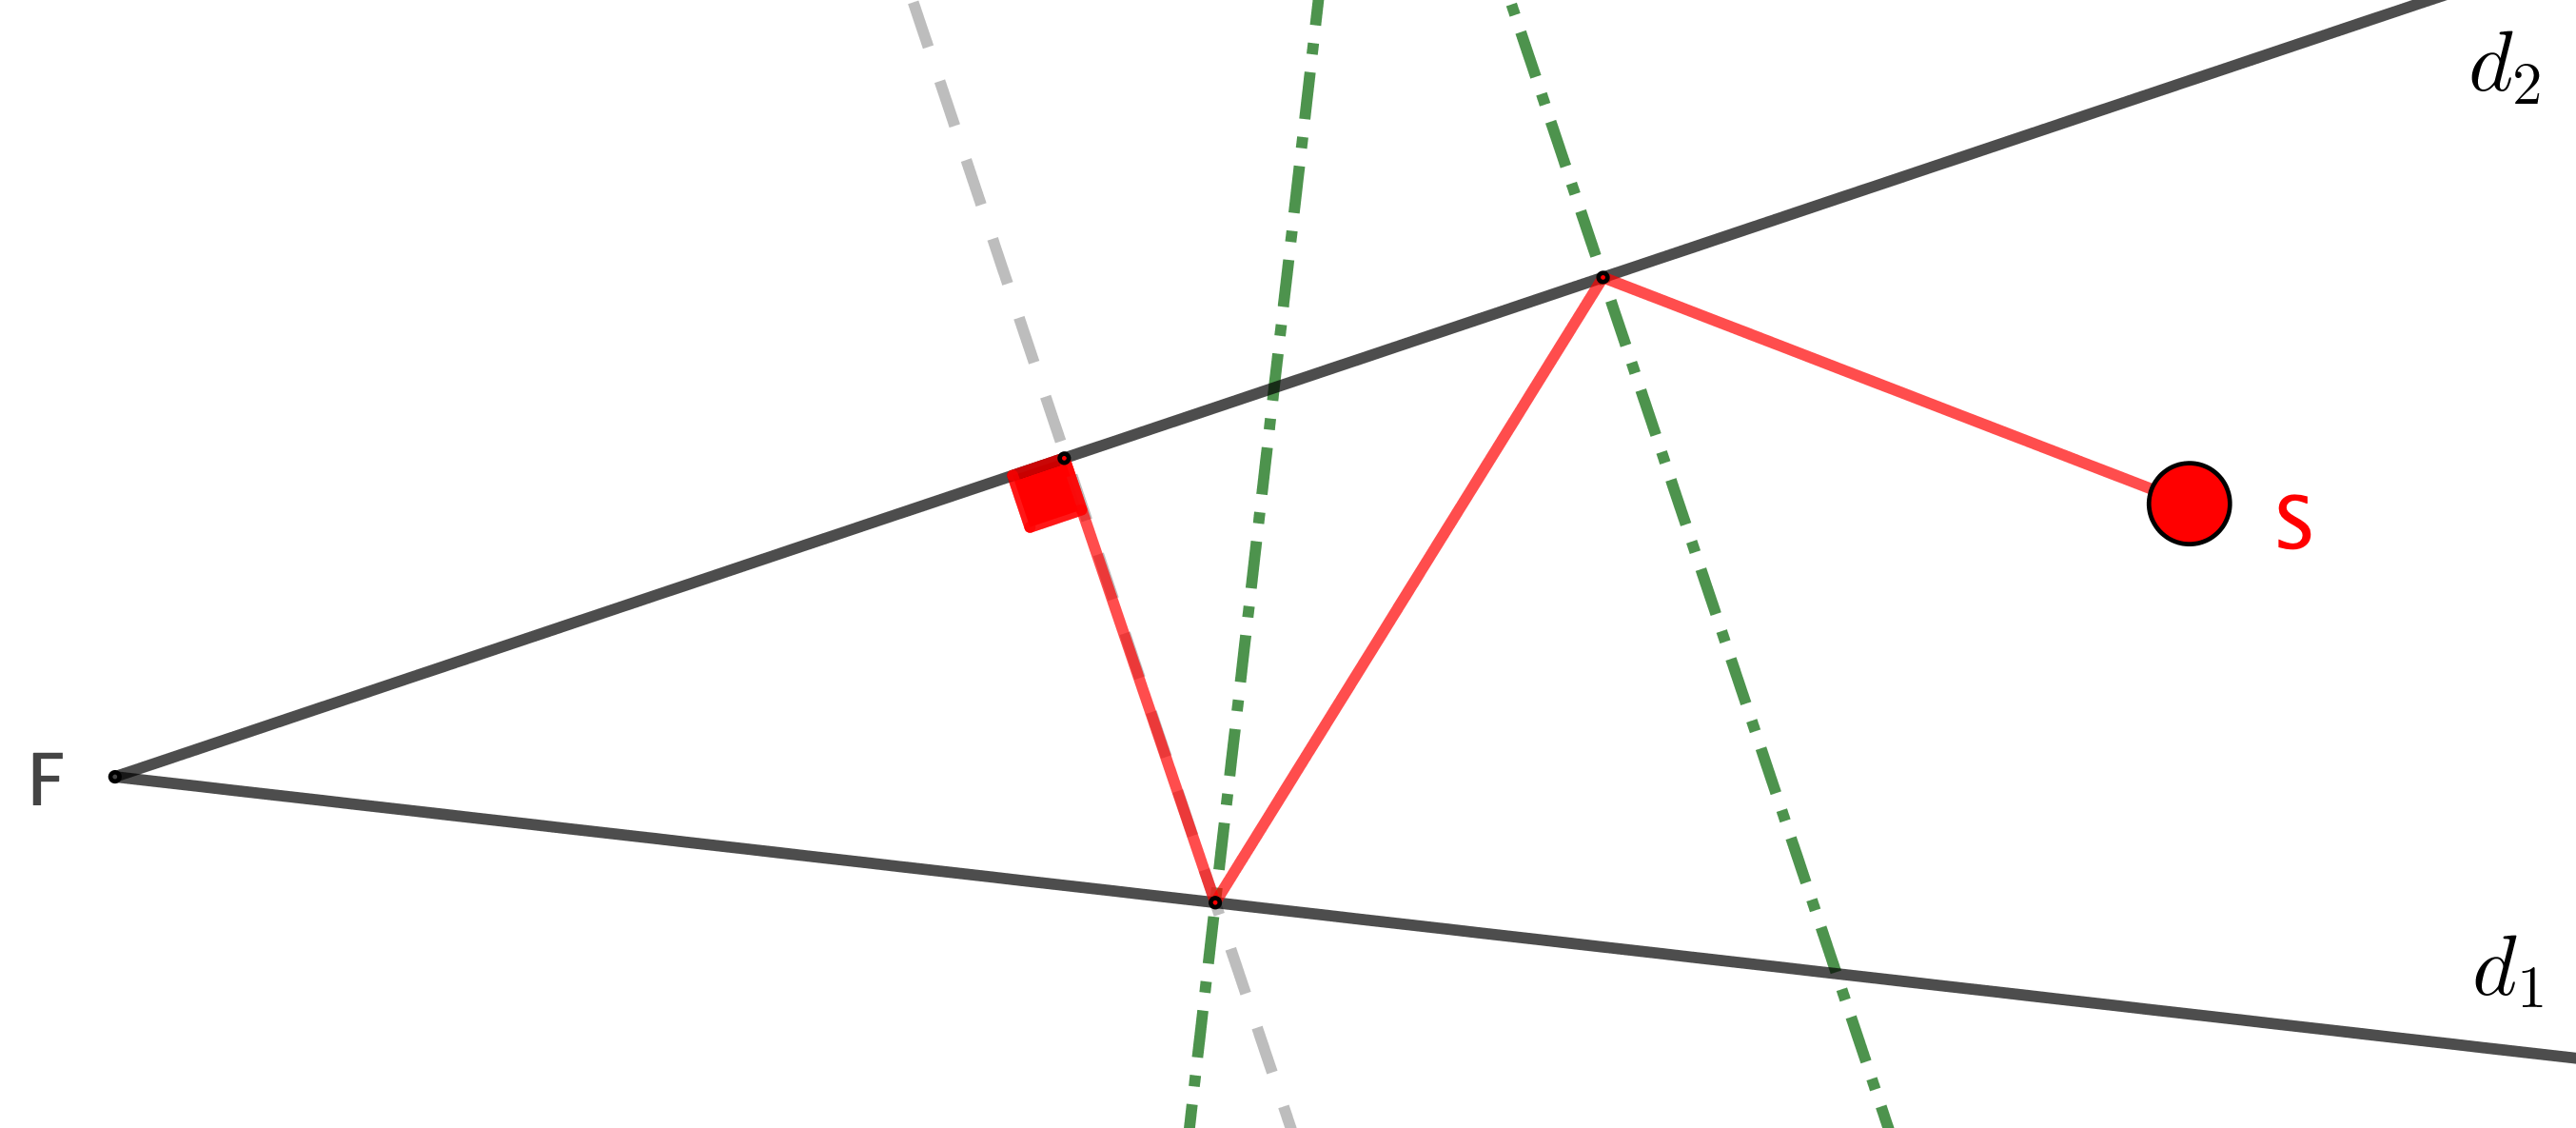
\includegraphics[width=12cm]{basic-math-pool/proof-starting-with-d2-2-bounces-to-ortho.png}

		\itshape\small
		Le 2\ieme{} rebond nous ramène à la situation du fait \ref{ortho-rebond} ci-dessus
		
		qui nous permet de conclure directement.
	\end{center}
	
	
	\medskip
	
	\begin{center}
		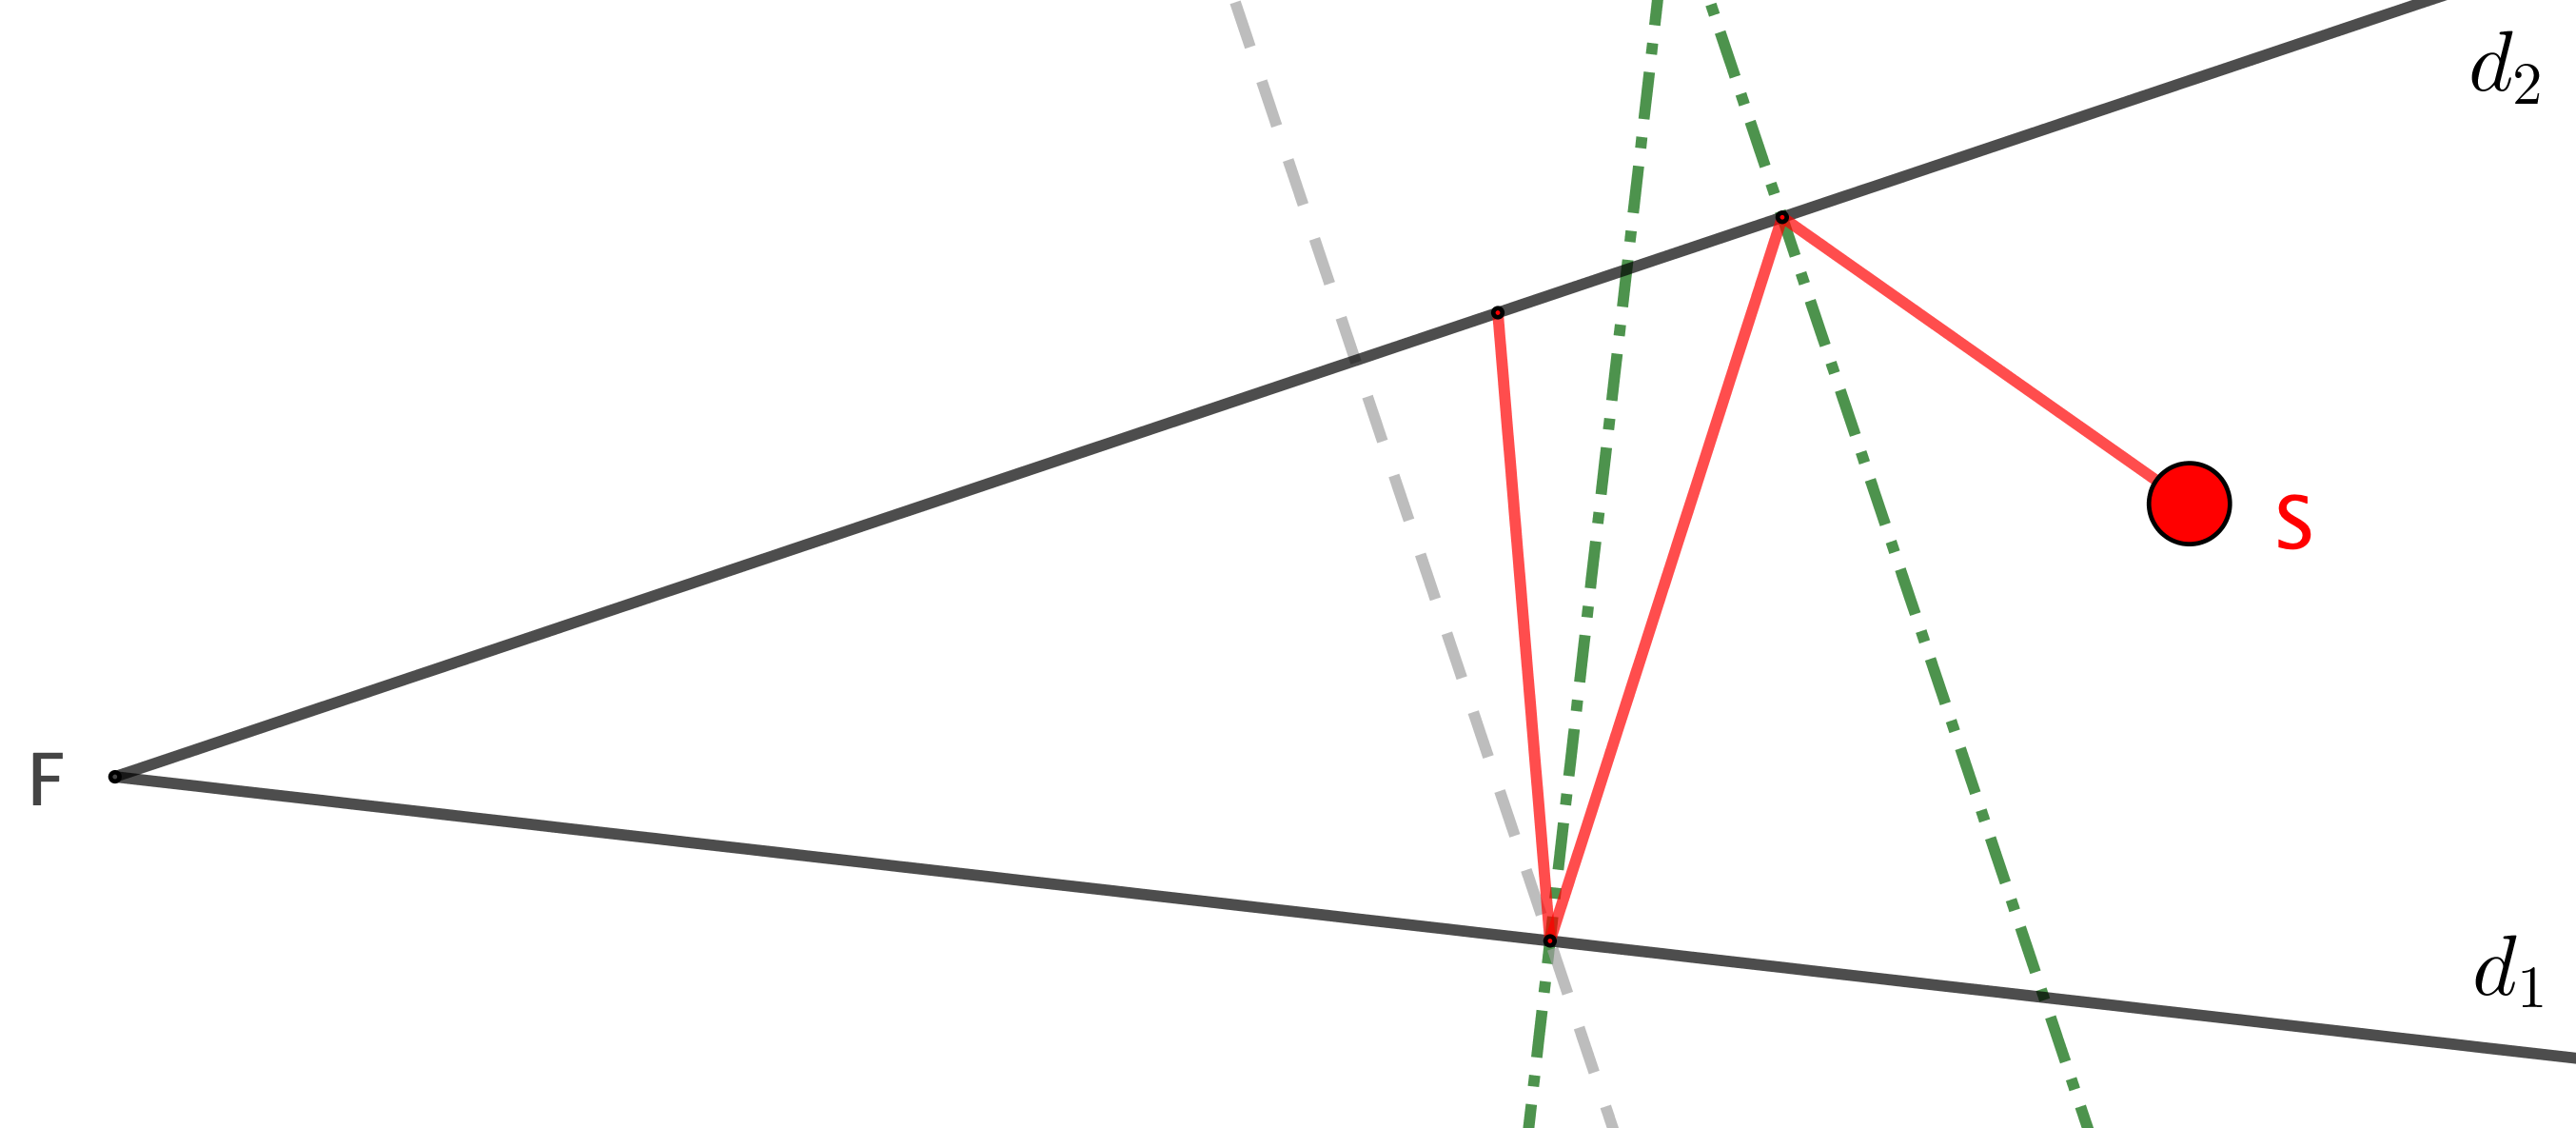
\includegraphics[width=12cm]{basic-math-pool/proof-starting-with-d2-2-bounces-to-infinity.png}

		\itshape\small
		Le 2\ieme{} rebond nous ramène directement à la bonne situation.
	\end{center}
	
	
	\medskip
	
	Voici la dernière situation représentée ci-dessous où $\setgeo{D}_2 \, /\!/ \, \setgeo{d}_2$.
	
	
	\medskip
	
	\begin{center}
		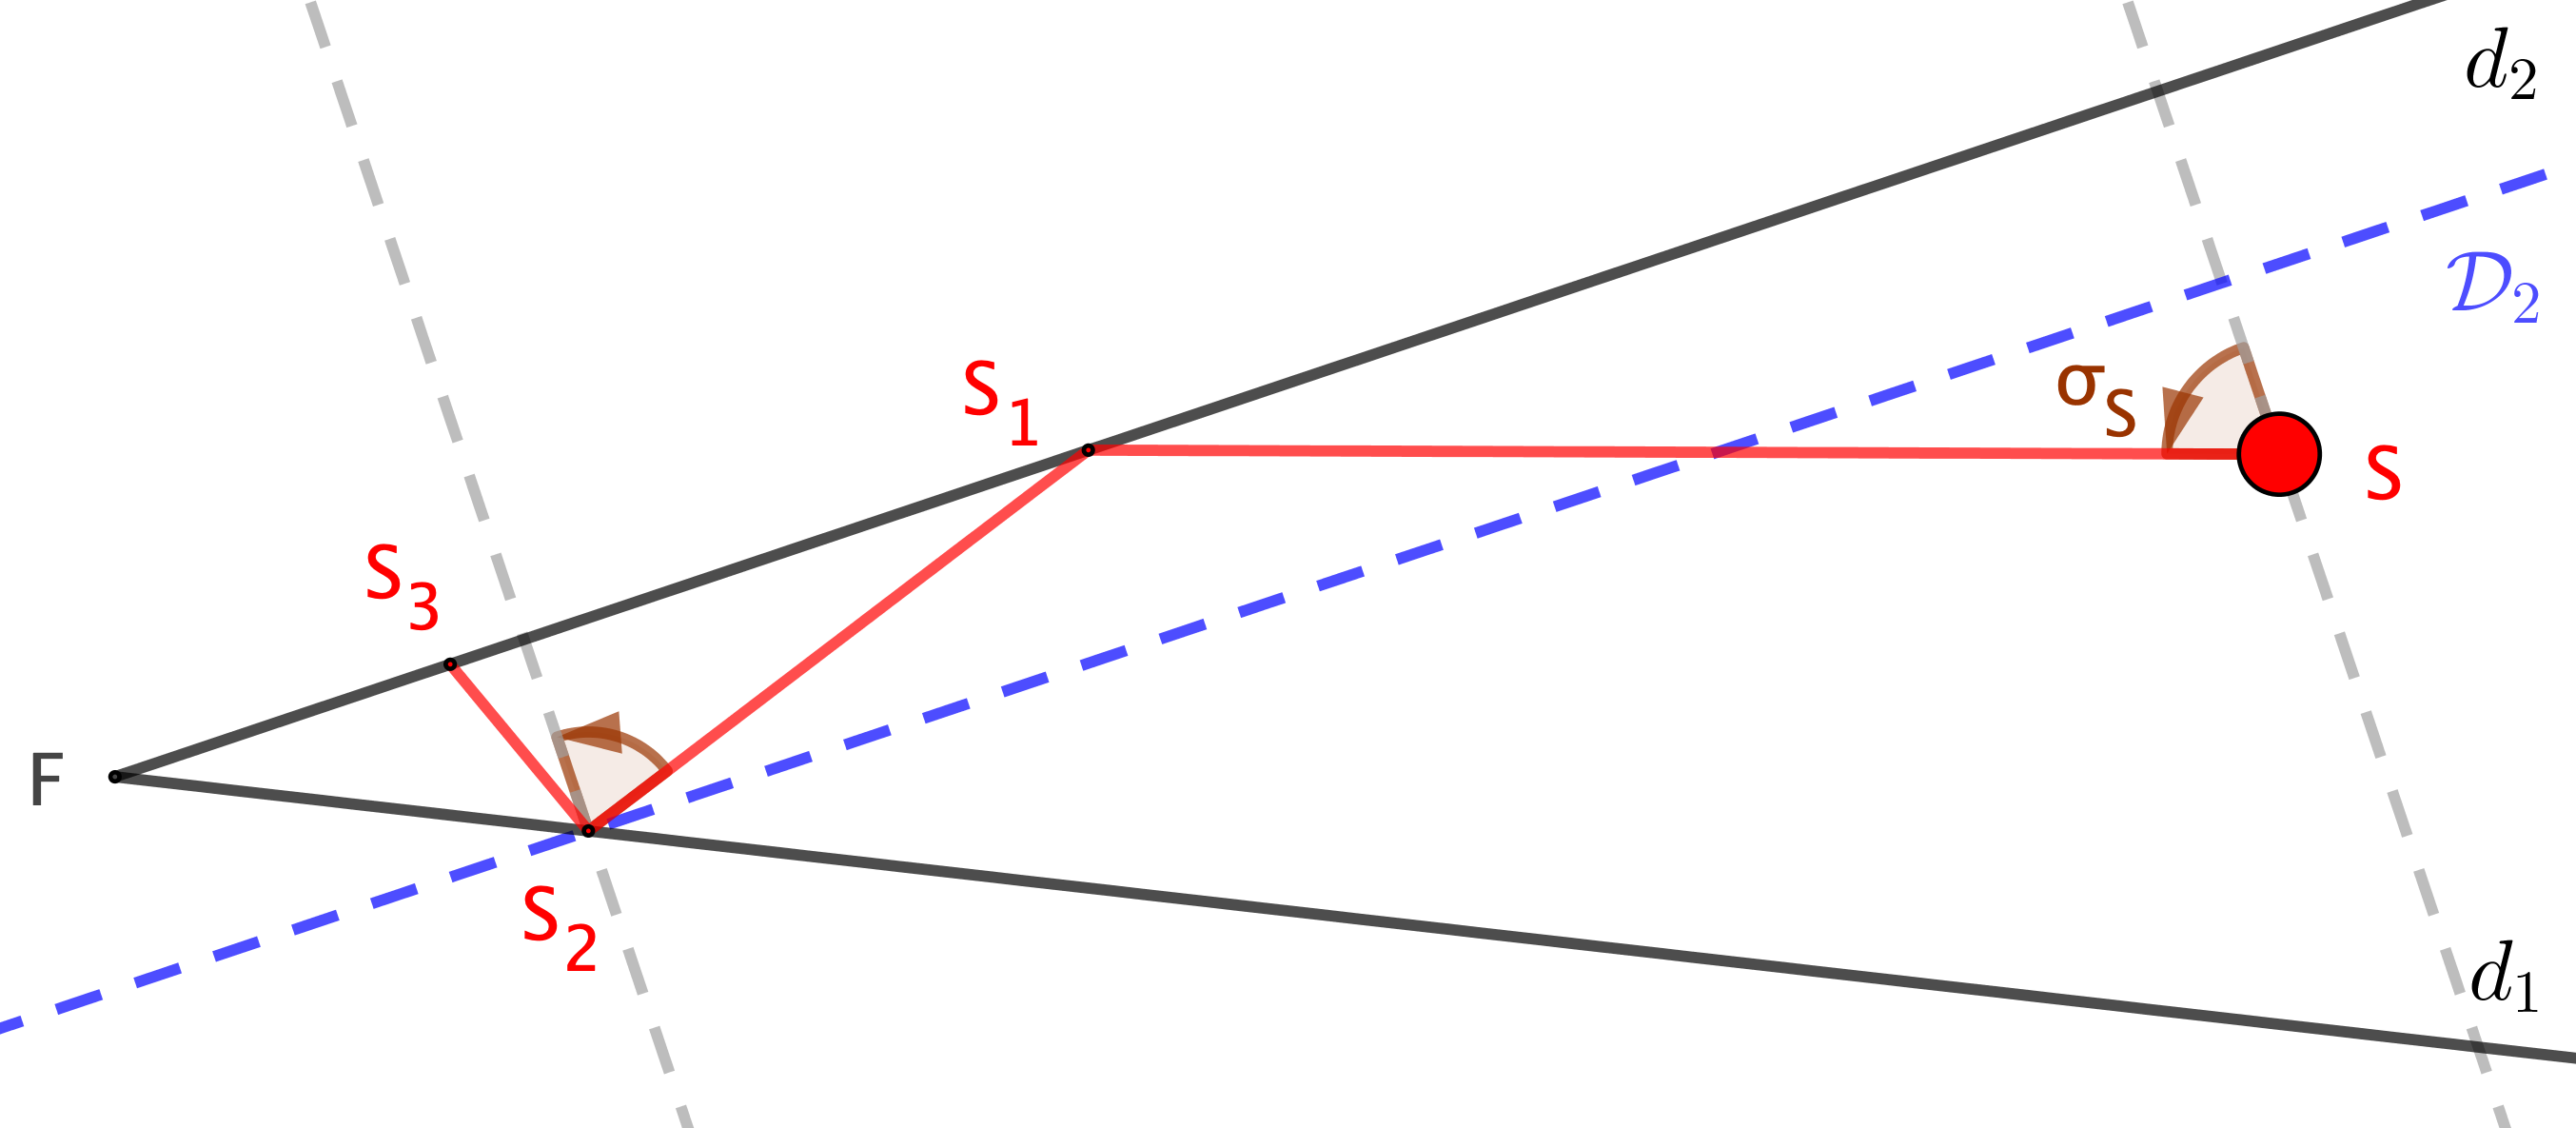
\includegraphics[width=12cm]{basic-math-pool/proof-starting-with-d2-2-bounces-to-F.png}

		\itshape\small
		Le 2\ieme{} rebond nous ramène à la situation de départ
		
		mais avec une valeur de $\sigma$ qui a augmenté.
	\end{center}
	
	
	\medskip
	
	Faisons un zoom sur la partie de gauche pour évaluer précisément l'évolution faisant passer de $\sigma_S$ à $\sigma_{S_2}$.
	
	\begin{center}
		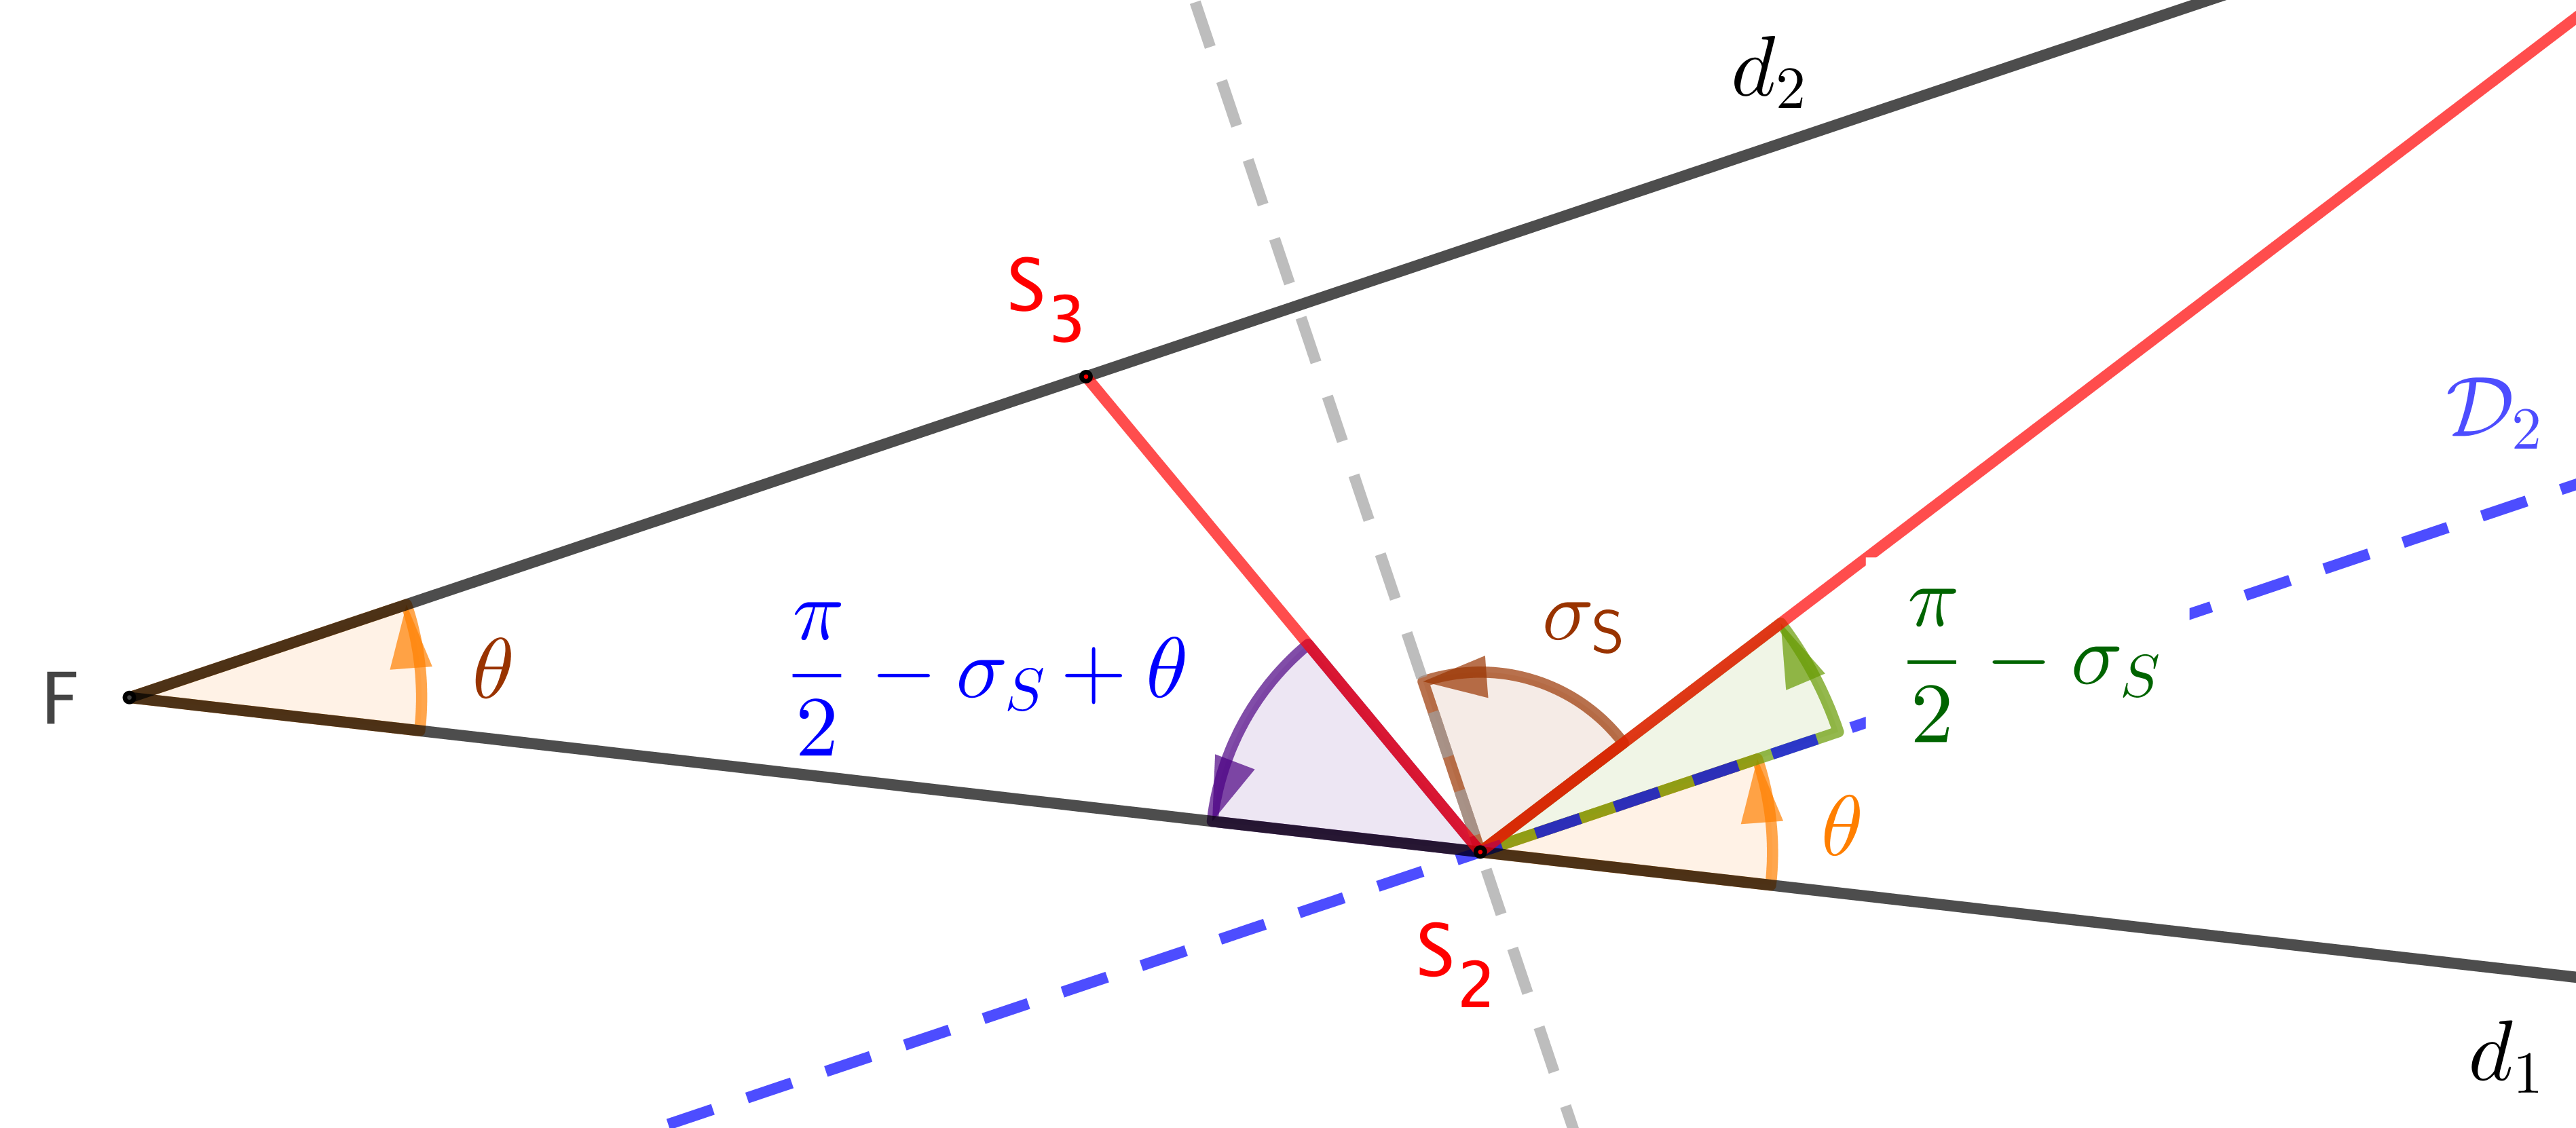
\includegraphics[width=12cm]{basic-math-pool/proof-starting-with-d2-2-bounces-to-F-zoom.png}
	\end{center}
	
	
	\medskip
	
	Nous avons alors $\sigma_{S_2} = \pi - 2 \left( \dfrac{\pi}{2} - \sigma_S + \theta \right) - \sigma_S = \sigma_S - 2 \theta$.
	Ceci montre que l'on passe de $\sigma_S$ à $\sigma_{S_2} = \sigma_S + \delta$ où $\delta = - 2 \theta < 0$. Cette dernière relation montre que l'on ne pourra pas avoir indéfiniment la dernière situation \emph{(en toute rigueur, il faudrait faire un raisonnement par récurrence)}.  
\end{proof}


\medskip


\begin{fact} \label{s-eloigner}
	Supposons que $\sigma_S \in \intervalCO{- \dfrac{\pi}{2}}{0}$.

	\medskip
	
	Il existe un point $M$ sur le trajet de la bille, mais pas sur $\setgeo*{d}{1}$, tel que $\sigma_M < - \dfrac{\pi}{2}$. En particulier, à partir de ce point $M$ la bille s'éloignera indéfiniment loin de $F$.
\end{fact}

\begin{proof}
	La démarche est similaire à la preuve précédente.
	Pour la situation problématique, on utilise les deux graphiques donnés dans la page suivante qui nous montrent que l'on passe de $\sigma_S$ à $\sigma_{S_2} = \sigma_S + \delta$ où $\delta = - 2 \theta < 0$. Ceci nous permet une seconde fois de conclure puisque l'on ne pourra pas avoir indéfiniment $\sigma_{S_{2k}} \geqslant - \dfrac{\pi}{2}$.
\end{proof}


\medskip


\begin{theorem}
	Si le 1\ier{} rebond se fait sur $\setgeo*{d}{2}$ alors il n'y aura qu'un nombre fini de rebonds et le dernier rebond amènera la bille à s'éloigner indéfiniment loin de $F$.
\end{theorem}

\begin{proof}
	Distinguons trois cas.
	
	\begin{itemize}[label = \textbullet]
		\item Si $\sigma_S \in \intervalCO{- \dfrac{\pi}{2}}{0}$ alors tout est donné par le fait \ref{s-eloigner}.


		\item Si $\sigma_S = 0$ alors le fait \ref{ortho-rebond} nous donne un point $M$ sur le trajet de la bille, mais pas sur $\setgeo*{d}{1}$, tel que $\sigma_M < 0$.
		
		\noindent
		Si $\sigma_M < - \dfrac{\pi}{2}$, nous savons qu'à partir de $M$ la bille s'éloignera indéfiniment loin de $F$.
		
		\noindent
		Sinon nous avons $\sigma_M \in \intervalCO{- \dfrac{\pi}{2}}{0}$.
		Le fait \ref{s-eloigner} nous permet alors de conclure.
		
		
		\item Enfin si $\sigma_S \in \intervalO{0}{\dfrac{\pi}{2} - \theta + \tau}$, il suffit de raisonner comme dans le point précédent mais en invoquant le fait \ref{deux-rebonds-vers-F}.
	\end{itemize}
\end{proof}

	
\medskip


\begin{center}
	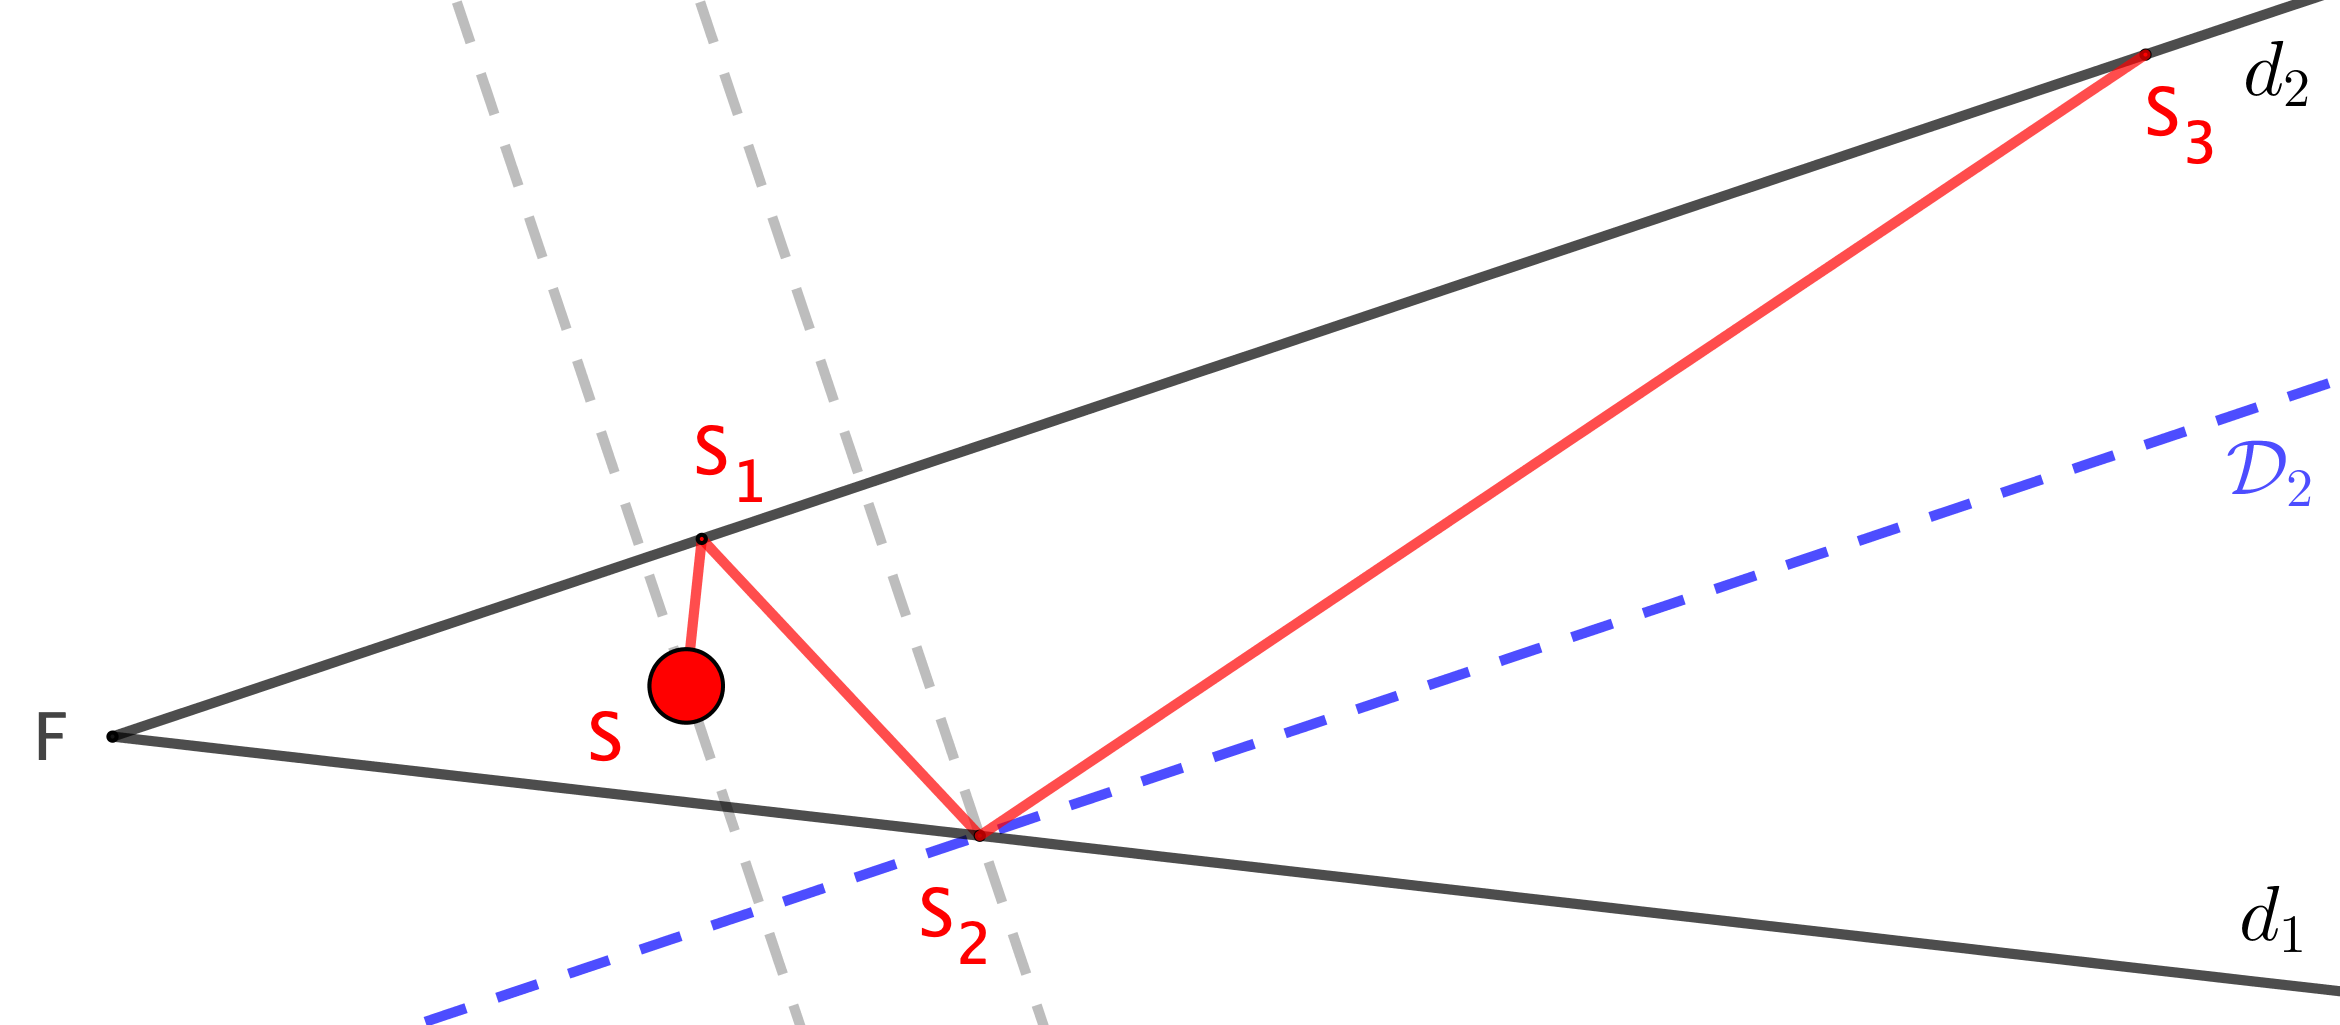
\includegraphics[width=12cm]{basic-math-pool/proof-starting-with-d2-2-bounces-farway-from-F.png}

	\itshape\small
	Preuve du fait \ref{s-eloigner} -- Vue large du cas problématique
\end{center}

	
\medskip


\begin{center}
	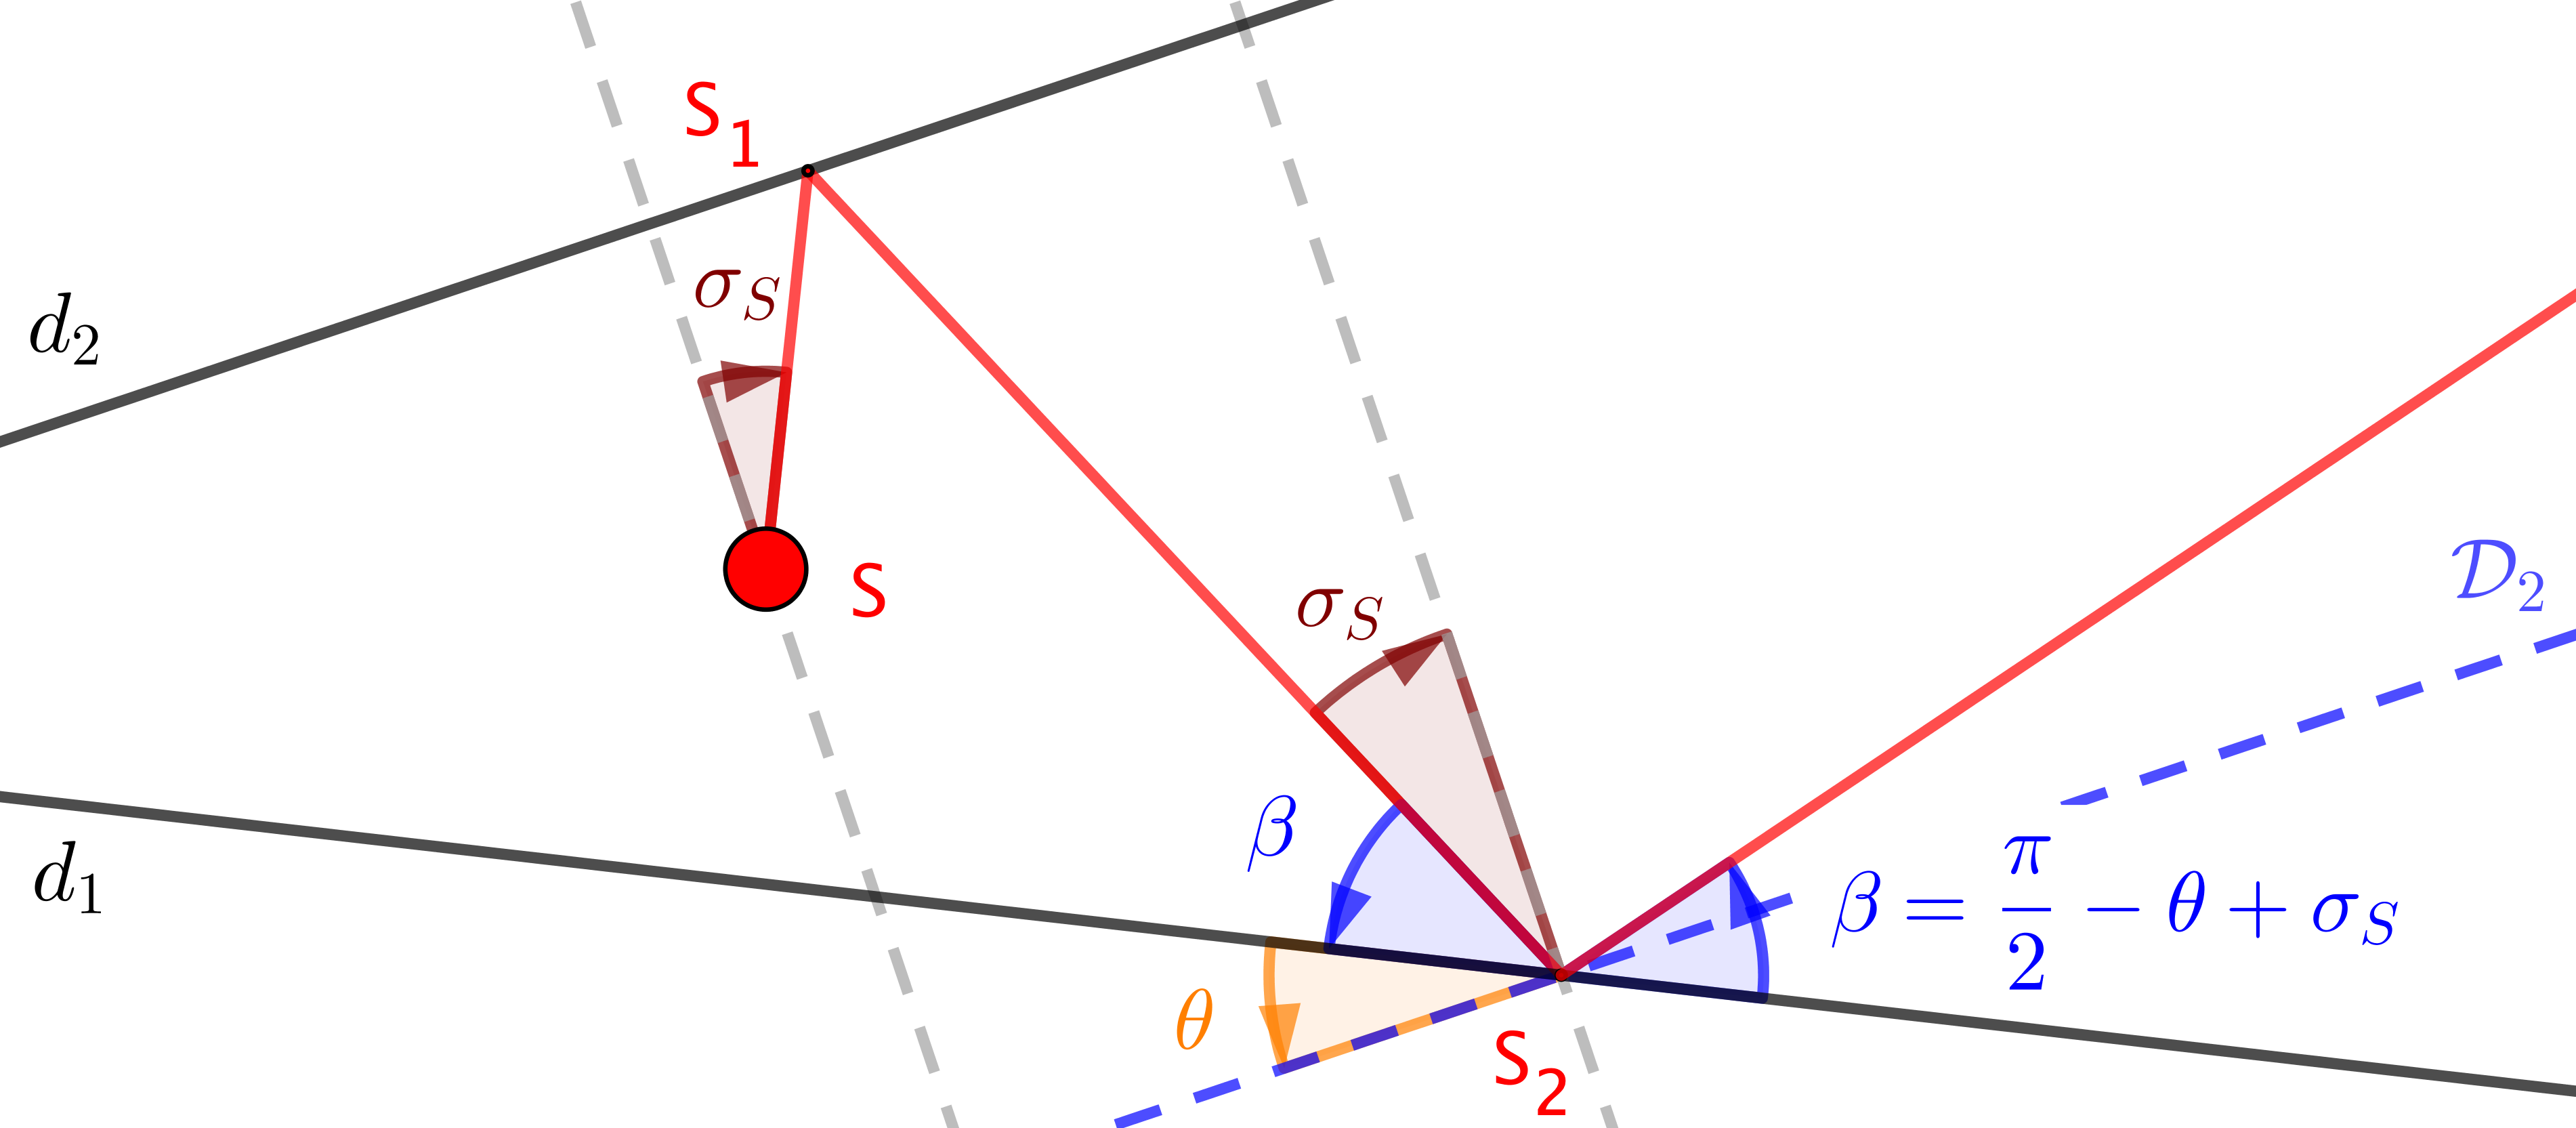
\includegraphics[width=12cm]{basic-math-pool/proof-starting-with-d2-2-bounces-farway-from-F-zoom.png}

	\itshape\small
	Preuve du fait \ref{s-eloigner} -- Vue zoomée du cas problématique
\end{center}



\end{document}
